\documentclass[12pt,a4paper]{article}

\usepackage[]{graphicx}
\usepackage{svg}
\usepackage[]{color}
\usepackage{alltt}
\usepackage{caption}
\usepackage{subcaption}
\usepackage{tabularx}
\usepackage{pdfpages}
\usepackage{booktabs}

\captionsetup[table]{position=above}
\newcommand{\mytitle}{Embedding optimization with deep neural networks for clustering image-based flow cytometry data}
\newcommand{\myname}{Dinesh Reddy Palli}
\newcommand{\mysupervisor}{Prof. Dr Fabian Theis}
\newcommand{\myinternalsupervisor}{PD Dr Michael Menden}

\usepackage[a4paper, width = 160mm, top = 35mm, bottom = 30mm, 
bindingoffset = 0mm]{geometry}
\usepackage[utf8]{inputenc}
\usepackage{xcolor}
\usepackage[numbers]{natbib}
\usepackage{fancyhdr}
\newcommand{\changefont}{%
    \fontsize{8}{11}\selectfont
}
\usepackage{hyperref}
\hypersetup{
  colorlinks = true,
  linkcolor = black,
  urlcolor = black,
  citecolor = black}
\pagestyle{fancy}

\fancyhead{}
\fancyhead[R]{\changefont{\mytitle}}
\fancyfoot{}
\fancyfoot[R]{\thepage}
\setlength{\headheight}{14.5pt}
\setlength{\parindent}{20pt}
\interfootnotelinepenalty = 10000
\captionsetup[figure]{font=small}

% ------------------------------------------------------------------------------
% MAIN -------------------------------------------------------------------------
% ------------------------------------------------------------------------------
\IfFileExists{upquote.sty}{\usepackage{upquote}}{}
\begin{document}

% FRONT PAGE -------------------------------------------------------------------
 
\begin{titlepage}
\begin{center}
    
\LARGE
Master's Thesis
    
\vspace{0.5cm}
      
\rule{\textwidth}{1.5pt}
\LARGE
\textbf{\mytitle}
\rule{\textwidth}{1.5pt}
   
\vspace{0.5cm}
      
\large
Department of Plant Sciences \\
Ludwig-Maximilians-Universität München 

\vfill

\Large
\textbf{\myname}

\vfill

\large
Munich, July 31\textsuperscript{st}, 2023
      
\vfill


\includegraphics[width = 0.4\textwidth]{Figures/sigillum.png}


\vfill

\normalsize
Submitted in partial fulfillment of the requirements for the degree of M. Sc.\\

Supervised by \mysupervisor{} \& \myinternalsupervisor

\end{center}
\end{titlepage}

\newpage

\includepdf{Attachments/quote.pdf}

% CONTENTS ---------------------------------------------------------------------

\pagenumbering{Roman}
\newpage

\newpage
\tableofcontents

%%% if you would want to include material overview
%%% use one of the following in addition
\newpage
\listoffigures
\newpage
\listoftables

\newpage

% CHAPTERS ---------------------------------------------------------------------

\pagenumbering{arabic}

\section{Abstract}
\label{Abstract}
\input{chapters/Abstract}

Advances in cell-sorting enable collection of high-dimensional images capturing cell morphological diversity. However analyzing these datasets to identify distinct cell phenotypes poses challenges. This study evaluates machine learning techniques for unsupervised clustering of cell images based on biologically-relevant traits without manual gating. We assess if classical image features contain sufficient information to separate cell types and states on Salmonella, phytoplankton and cell cycle datasets. While providing preliminary separations, hand-engineered features lack complexity to capture nuanced morphological patterns denoting phenotypic variations. We check pretrained deep convolutional networks, evaluating the performance of the same. However, by training vision transformers end-to-end on datasets, we demonstrate deep learning's potential to learn specialized features when optimized on relevant data. We are optimistic that with rigorous tuning, deep neural networks can uncover new biology from high-dimensional imaging datasets in an automated manner.
    
\section{Introduction}
\label{intro}
\input{chapters/introduction}
\subsection{Background}

In biomedical sciences, understanding the connection between genetic variation and phenotypic diversity is of paramount importance. This relationship forms the foundation for deciphering the principles of cellular function, identifying the causes and markers of diseases, and is crucial for biological engineering and synthetic biology applications. These applications range from library screening for the development of new protein biosensors, transcriptional reporters, synthetic enzymes, RNA devices, genetic circuits, signaling pathways, to multicellular communities. High-throughput screening approaches are highly desirable in these contexts, as they allow for the efficient identification of variants exhibiting the properties of interest from heterogeneous populations of cells \cite{Pegoraro2017-rs}.

Methods that physically separate cells based on measurable characteristics have a wide range of uses in both research and clinical applications, including cellular therapies. Techniques such as microfluidics, filters, and centrifugation can identify and physically separate cells from a heterogeneous population according to intrinsic characteristics like size, shape, and deformability \cite{https://doi.org/10.1002/bit.22833}. Additionally, cells can be sorted based on signals from extrinsic probes. These techniques, when combined with high-throughput screening approaches, provide a powerful toolset for mapping genotypes to phenotypes, thereby advancing our understanding of genetic variation and its impact on phenotypic diversity \cite{vandereyken_sifrim_thienpont_voet_2023}. One of the most popular technique in sorting cells based on their characteristics, is Fluorescent Assisted Cell Sorting. FACAS is based on Flow Cytometry \cite{liao_makris_luo_2016}.

\subsection{Flowcytometry \& Fluorescence Microscopy}

Flow cytometry is a technique used to analyze the physical and chemical properties of particles, usually cells as they flow through a laser beam. Flow cytometry uses the light properties scattered from cells or particles for identification or quantitative measurement of physical properties \cite{mckinnon_2018}. Labels, dyes, and stains can be used for multi-parametric analysis including size, shape, and the expression of specific proteins or other cellular components. The principle behind flow cytometry is the use of laser light to excite fluorescently labeled particles, which then emit light at specific wavelengths. The emitted light is collected and quantified using detectors, providing information on the characteristics of each cell or particle. Flow cytometry can sort cells based on their physical or chemical characteristics \cite{mckinnon_2018}. This is useful for isolating specific cell types from a heterogeneous population of cells, or for preparing cells for further analysis.

\begin{figure}
  \centering
  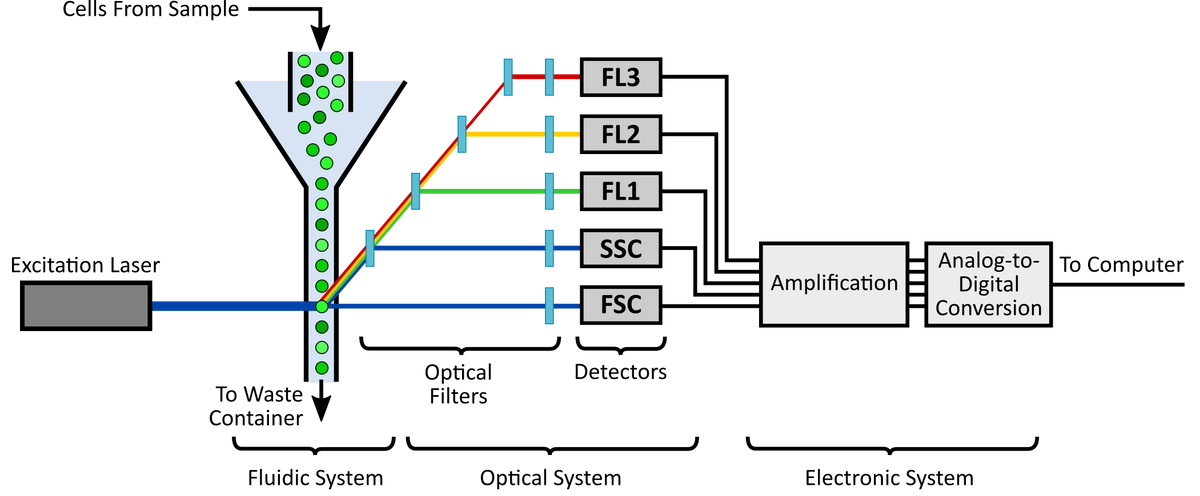
\includegraphics[width=\textwidth]{Figures/flow-cytometer.png}
  \caption{Diagrammatic representation of a typical flow cytometer. The figure illustrates the integration of the fluidic, optical, and electronic systems within the cytometer. The fluidic system guides the sample particles in a stream, the optical system illuminates the sample and collects the emitted light, and the electronic system converts the collected light into digital data for further analysis. \cite{aatbioFundamentalsFlow}}
  \label{flowcytometry}
\end{figure}

Fluorescence microscopy is a technique that uses fluorescence to generate an image of a sample. It is often used in biology to study the distribution of molecules in cells and tissues. The basic principle of fluorescence microscopy is that when light of a specific wavelength is shone on a fluorophore, the fluorophore absorbs the light and emits light of a longer wavelength. This emitted light is used to generate images of the samples \cite{sanderson_smith_parker_bootman_2014}.

\begin{figure}
  \centering
  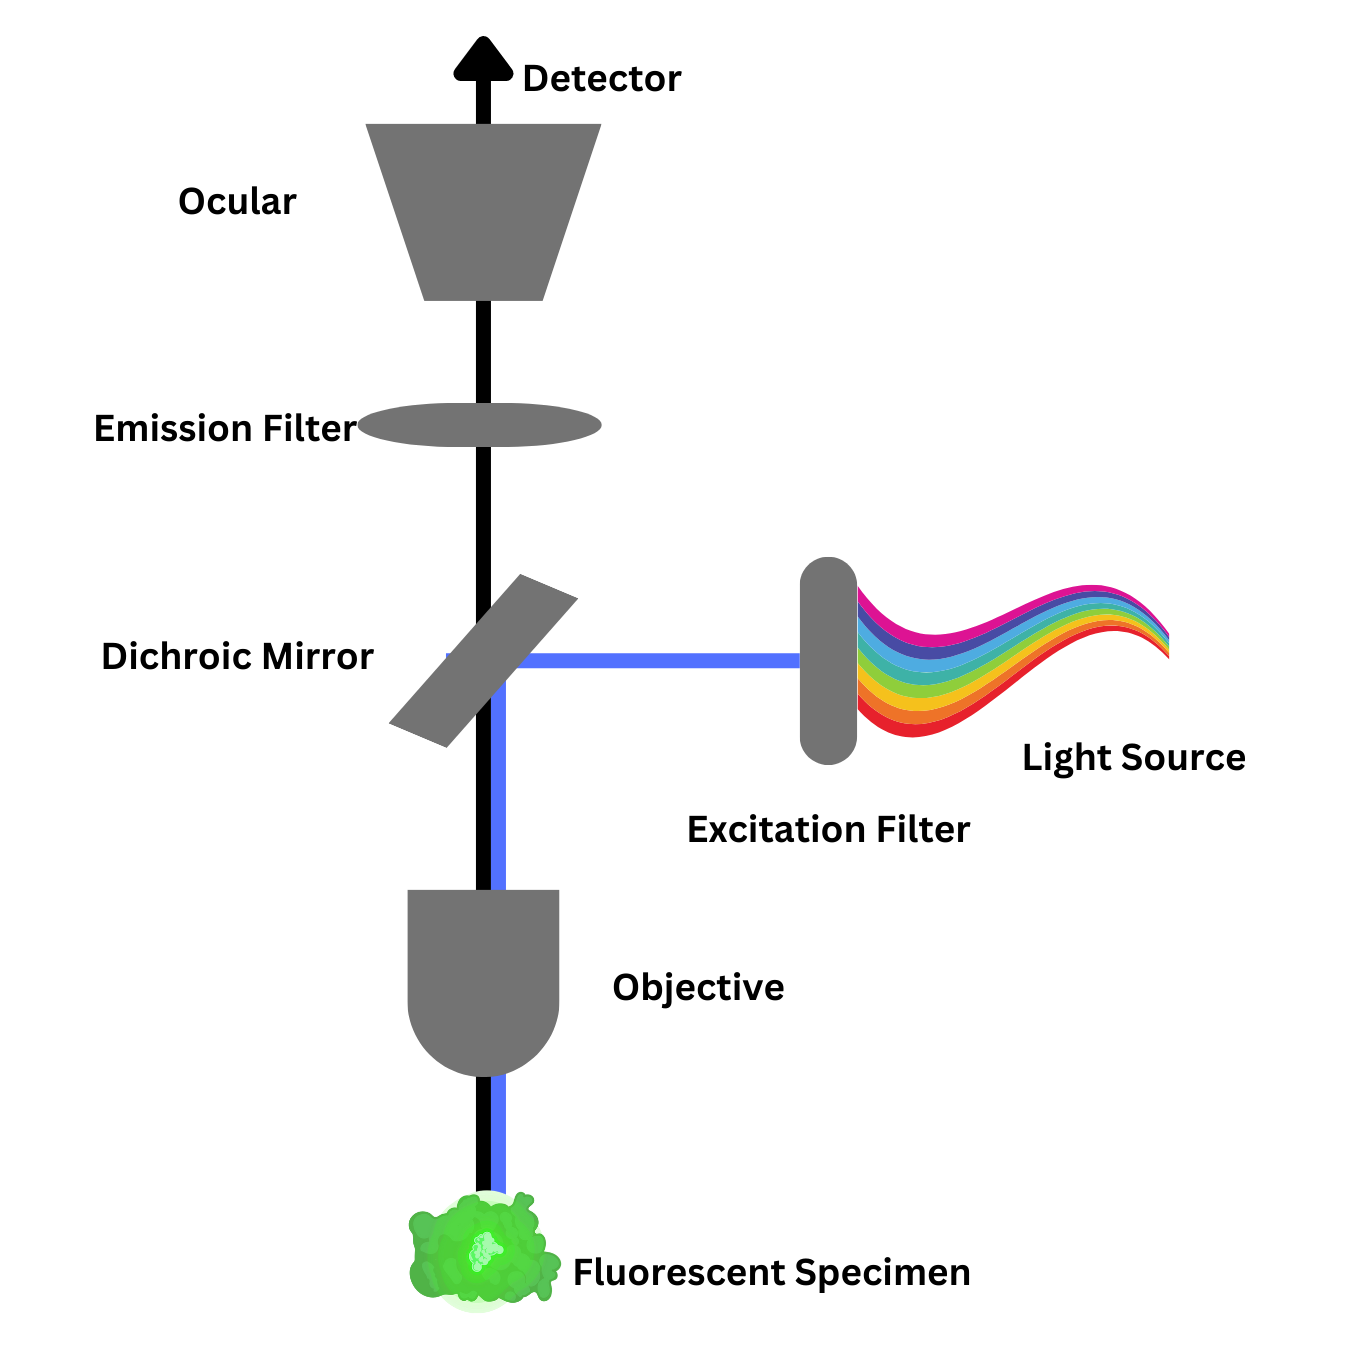
\includegraphics[width=0.3\textwidth]{Figures/454px-Fluorescence_Microscopy_01.png}
  \caption{A fluorescence microscope uses a light source to excite fluorescent molecules in a sample. The emitted light is then filtered and focused to create an image. The image shows a diagram of a fluorescence microscope. The light source is a mercury lamp, which emits a broad spectrum of light. The excitation filter only allows light of a certain wavelength to pass through. The dichroic mirror reflects the excitation light away and allows the fluorescent light to pass through. The emission filter only allows light of a certain wavelength to pass through. The objective lens focuses the fluorescent light onto the detector, which converts it into an image. \cite{File:Fluorescence Microscopy 01.png - Biology Wiki}}
  \label{fluorescencemicroscopy}
\end{figure}


\subsection{Image-Enabled Cell Sorter}
Flow cytometry and fluorescence microscopy are commonly used techniques in biological and biomedical research. While flow cytometry allows for the rapid and high-throughput isolation of cells based on low-dimensional parameters, it lacks the subcellular resolution needed to study processes such as protein trafficking, cellular signaling, or protein mislocalization during disease \cite{cossarizza_chang_radbruch_acs_adam_adamklages_agace_aghaeepour_akdis_allez_et_al._2019}. On the other hand, fluorescence microscopy provides high-resolution imaging of cellular morphology and protein localization, but it is not capable of quickly isolating cells with specific phenotypes \cite{Espina2006-iv}. Combining the spatial resolution of fluorescence microscopy with the sorting capabilities of flow cytometry has the potential to revolutionize experimental approaches by enabling the rapid identification and isolation of cells with specific sub-cellular phenotypes \cite{doi:10.1126/science.abj3013}.

Daniel Schraivogel et al. presented a system that integrates flow cytometry and microscopy, operates at high speeds suitable for genetic screening and the analysis of short-lived dynamic phenomena, and can be used in non-specialized laboratories \cite{doi:10.1126/science.abj3013}. This is referred to as image-enabled cell sorting (ICS). Traditional flow cytometry is able to distinguish between three stages of the cell cycle (G1, G2/mitosis, and S phase), but is unable to differentiate between cells in different stages of mitosis \cite{doi:10.1126/science.abj3013}. This was made possible with ICS. Here, we refer to the features maximum intensity, radial movement, eccentricity and other features mentioned in the study by Daniel Schraivogel et al. as the classical image features.


\begin{figure}
  \centering
  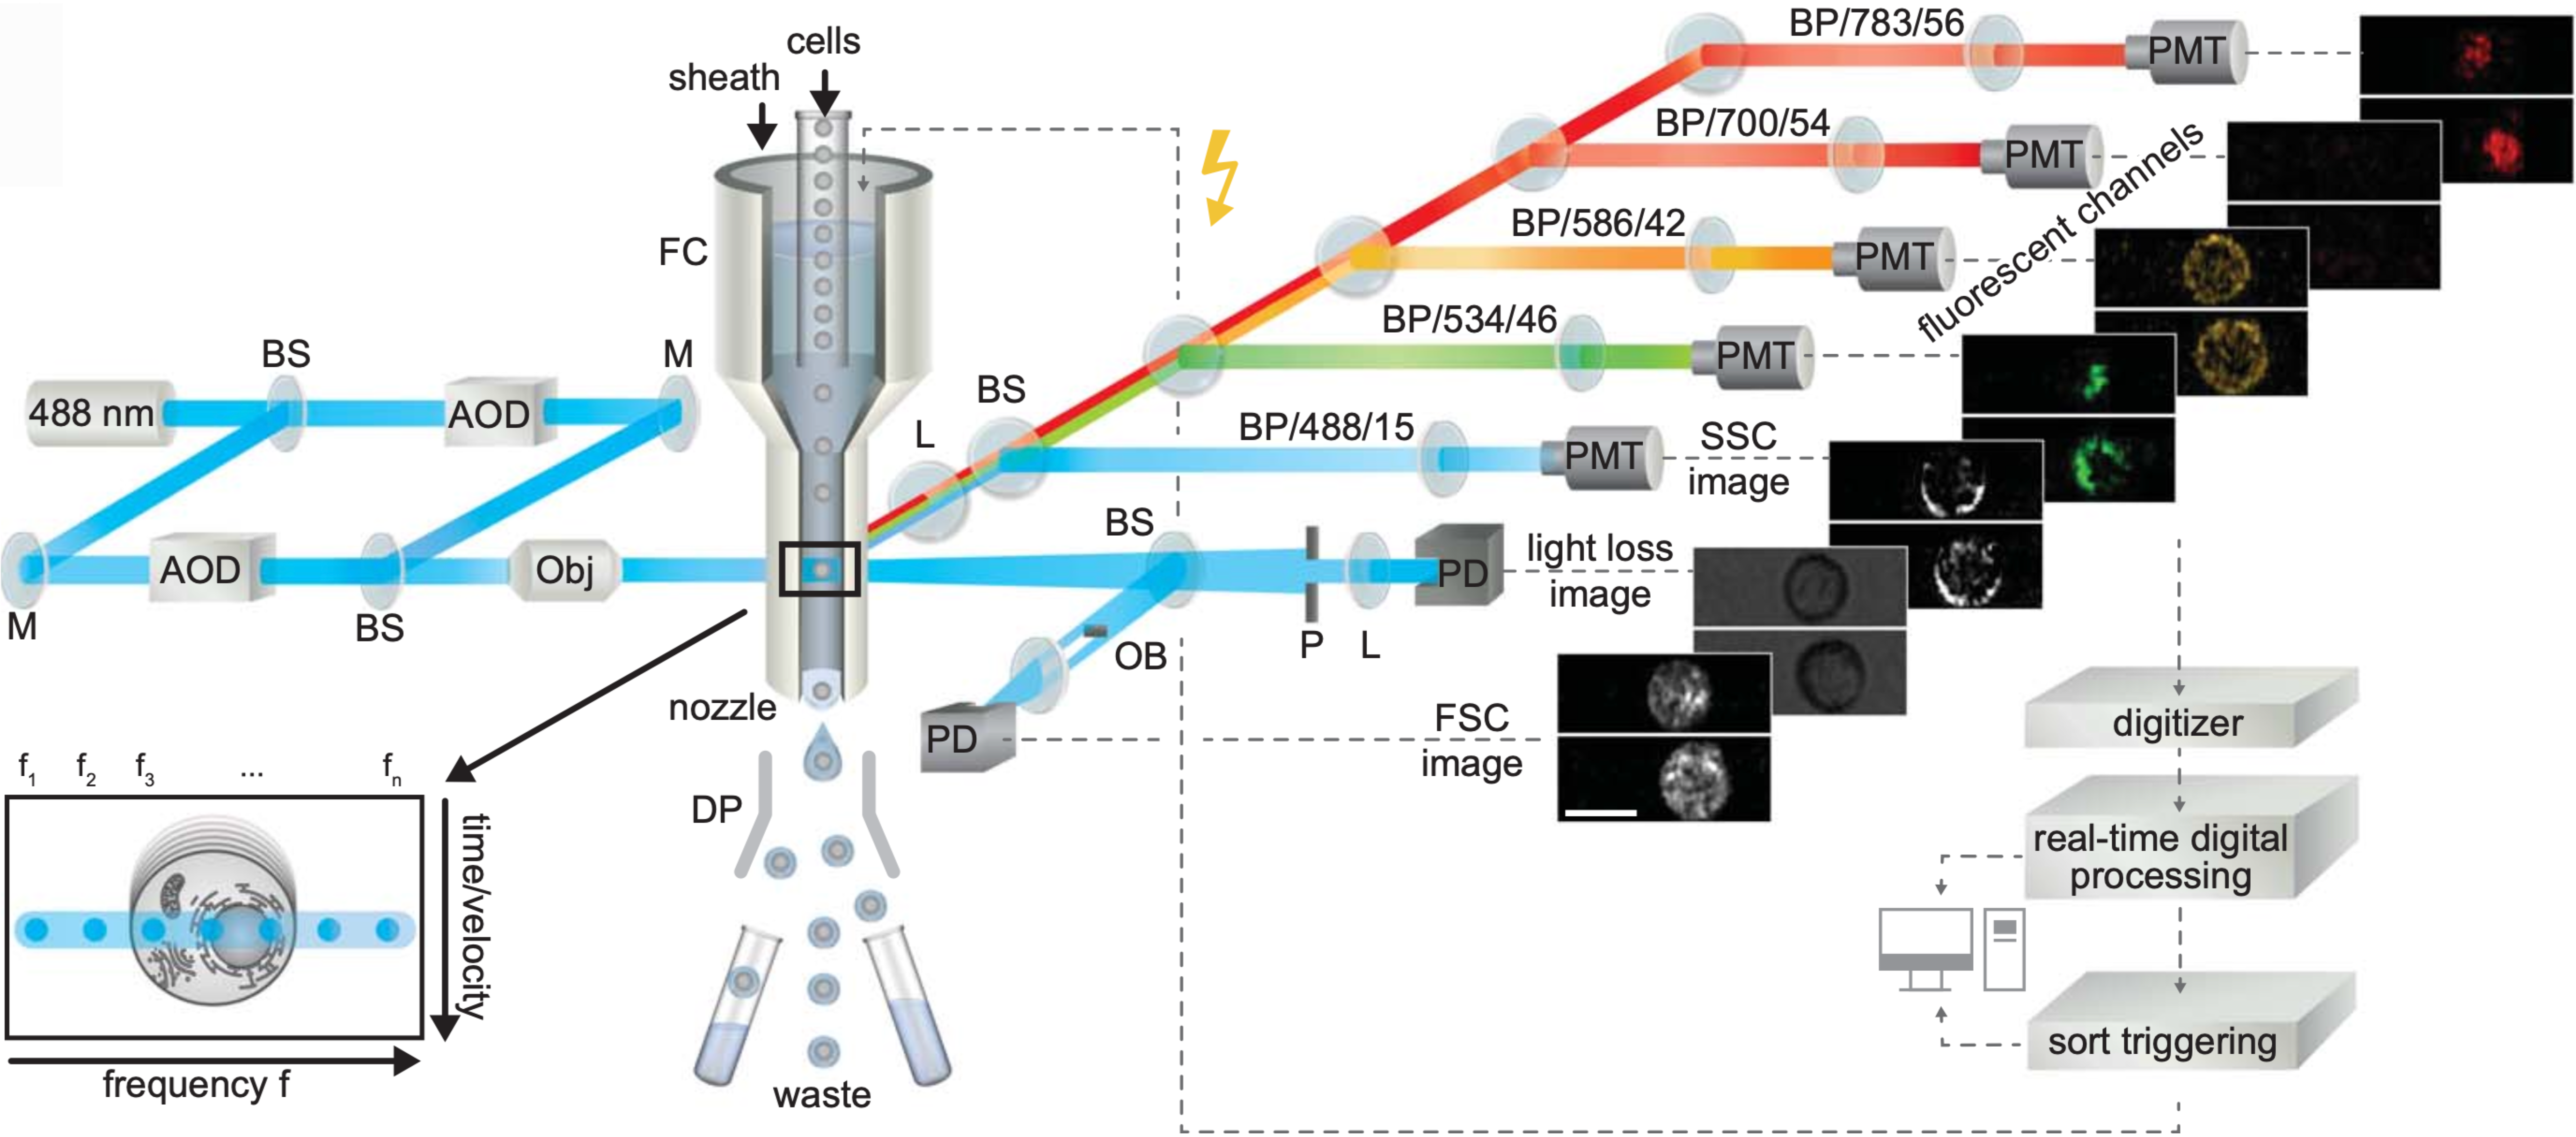
\includegraphics[width=\textwidth]{Figures/ICS_working.png}
  \caption{Schematic representation of the ICS optical and flow hardware components, showing the excitation and emission beam paths. The excitation beam path utilizes acousto-optic deflectors (AOD) to split a single laser beam into an array of beamlets with different optical frequencies and angles. Another AOD adjusts the optical frequency of a reference beam, which overlaps with the beamlet array. These overlapping beams intersect the flow cell (FC) of a cuvette sorter. The emission beam path involves generating images from digitized signals, including light loss, forward scatter (FSC), side scatter (SSC), and four fluorescent channels. Example images demonstrate the labeling of HeLa cells expressing GalNAcT2-green fluorescent protein (GFP) with CD147 PE-CF594 and DRAQ5 nuclear dye. Grayscale images display FSC, SSC, and light loss. The components used include beam splitter (BS), mirror (M), objective (Obj), deflection plates (DP), obscuration bar (OB), pinhole (P), lens (L), band pass (BP), photomultiplier tube (PMT), and photodiode (PD). Scale bar: 20 mm \cite{doi:10.1126/science.abj3013}.}
  \label{icsworking}
\end{figure}



\subsection{Complex Embedding is Required for Clustering ICS-Generated Data}
Flow cytometry data typically involves gating strategy - a step where a series of gates are defined to identify the population of interest. Manual gating typically involves two-dimensional plots for cell-type marker intensity and uses hierarchical gates to identify cell populations \cite{10.3389/fimmu.2021.787574}. The method of using 2D plots for analyzing flow cytometry data is sufficient for small experiments. But the problem arises when experiments have more measured parameters \ref{mair_hartmann_mrdjen_tosevski_krieg_becher_2016}. The main issue is that 2D plots do not scale up well. When there are more cell markers, the number of plots needed grows exponentially. For example, an experiment with 18 markers would need 153 different 2D plots to show all combinations. That many plots becomes too complex to comprehend and interpret \ref{mair_hartmann_mrdjen_tosevski_krieg_becher_2016}.

ICS produces high-dimensional single-cell data for which high-dimensional data analysis is needed, contradictory to manual gating in conventional flow cytometry as two-dimensional plots are unable to depict the complex high-dimensional structure of the data generated by the ICS \cite{doi:10.1126/science.abj3013}. The image features produced by the ICS, from the images, requires complex embedding on which clustering can be done. In machine learning, embedding refers to the process of representing complex, high-dimensional data in a lower-dimensional space, typically as continuous vectors. This makes it easier for computers to process and learn from data.

\begin{figure}
  \centering
  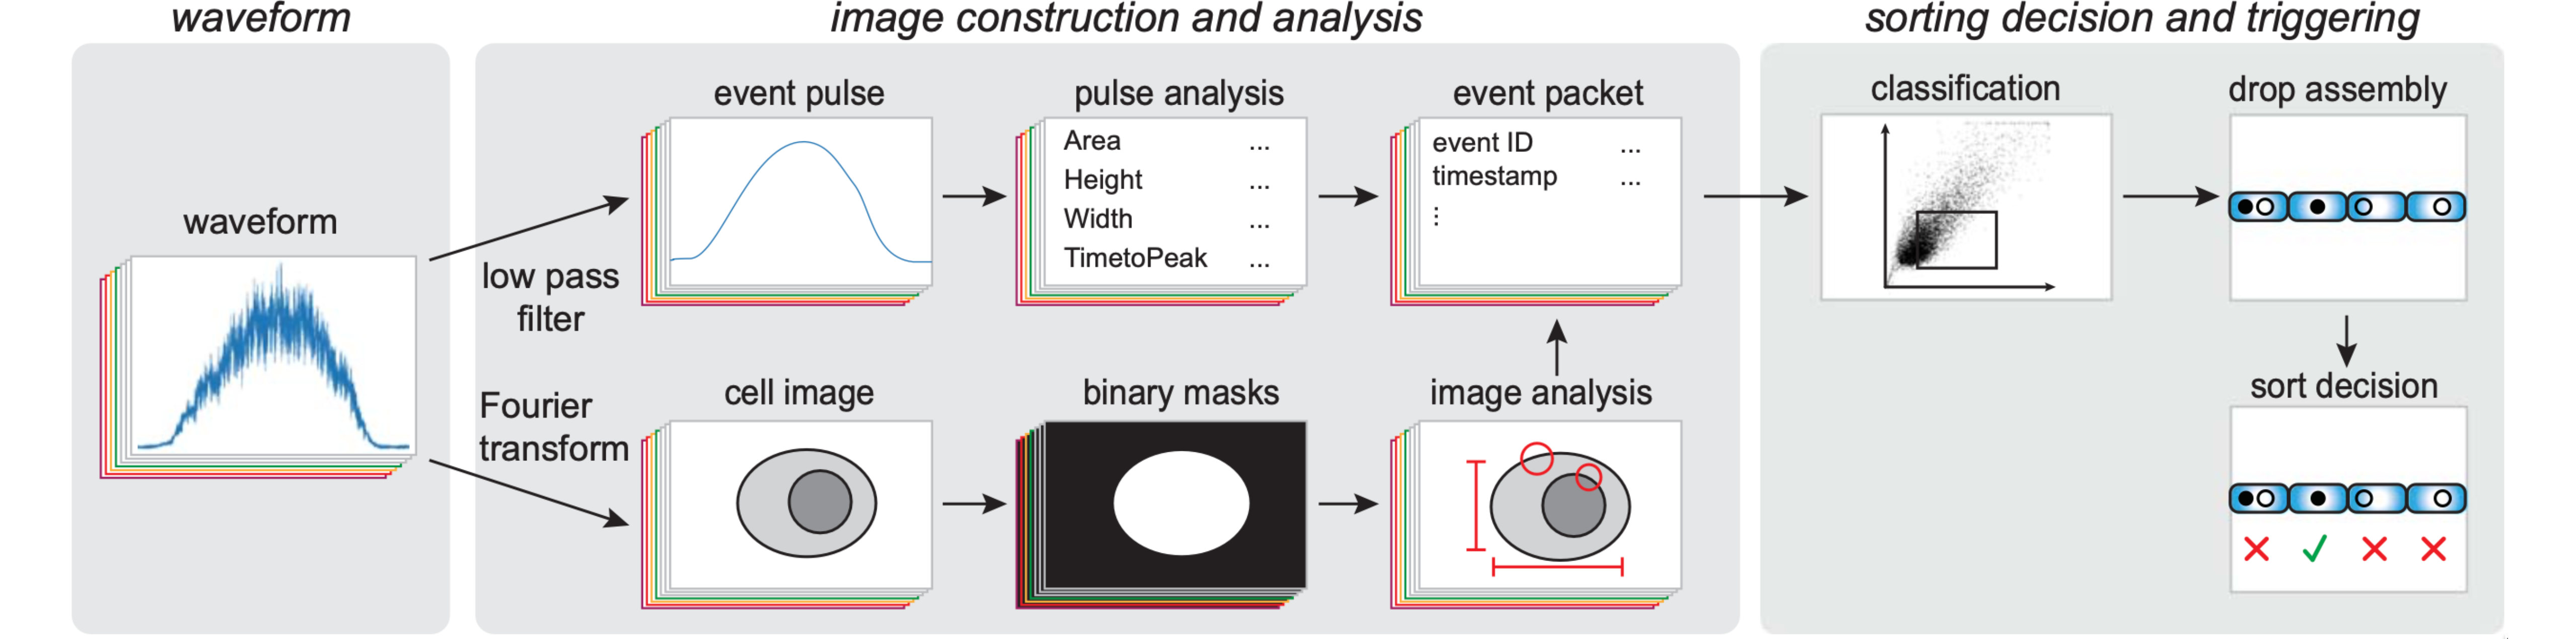
\includegraphics[width=\textwidth]{Figures/DataProcessingPipelineICS.png}
  \caption{Overview of the ICS low-latency data-processing pipeline, highlighting the steps involved. Photodetectors generate pulses with high-frequency modulations that encode the image waveform. Fourier analysis is employed to reconstruct the image from the modulated pulse. An image-processing pipeline extracts image features, while a pulse-processing pipeline derives additional features from the pulse. Real-time sort classification electronics utilize these features to classify particles and make sort decisions. The resulting sort decision is used to selectively charge the droplets, as indicated by the dotted gray line in panel A \cite{doi:10.1126/science.abj3013}.}
  \label{icsdataprocessing}
\end{figure}


\begin{figure}
  \centering
  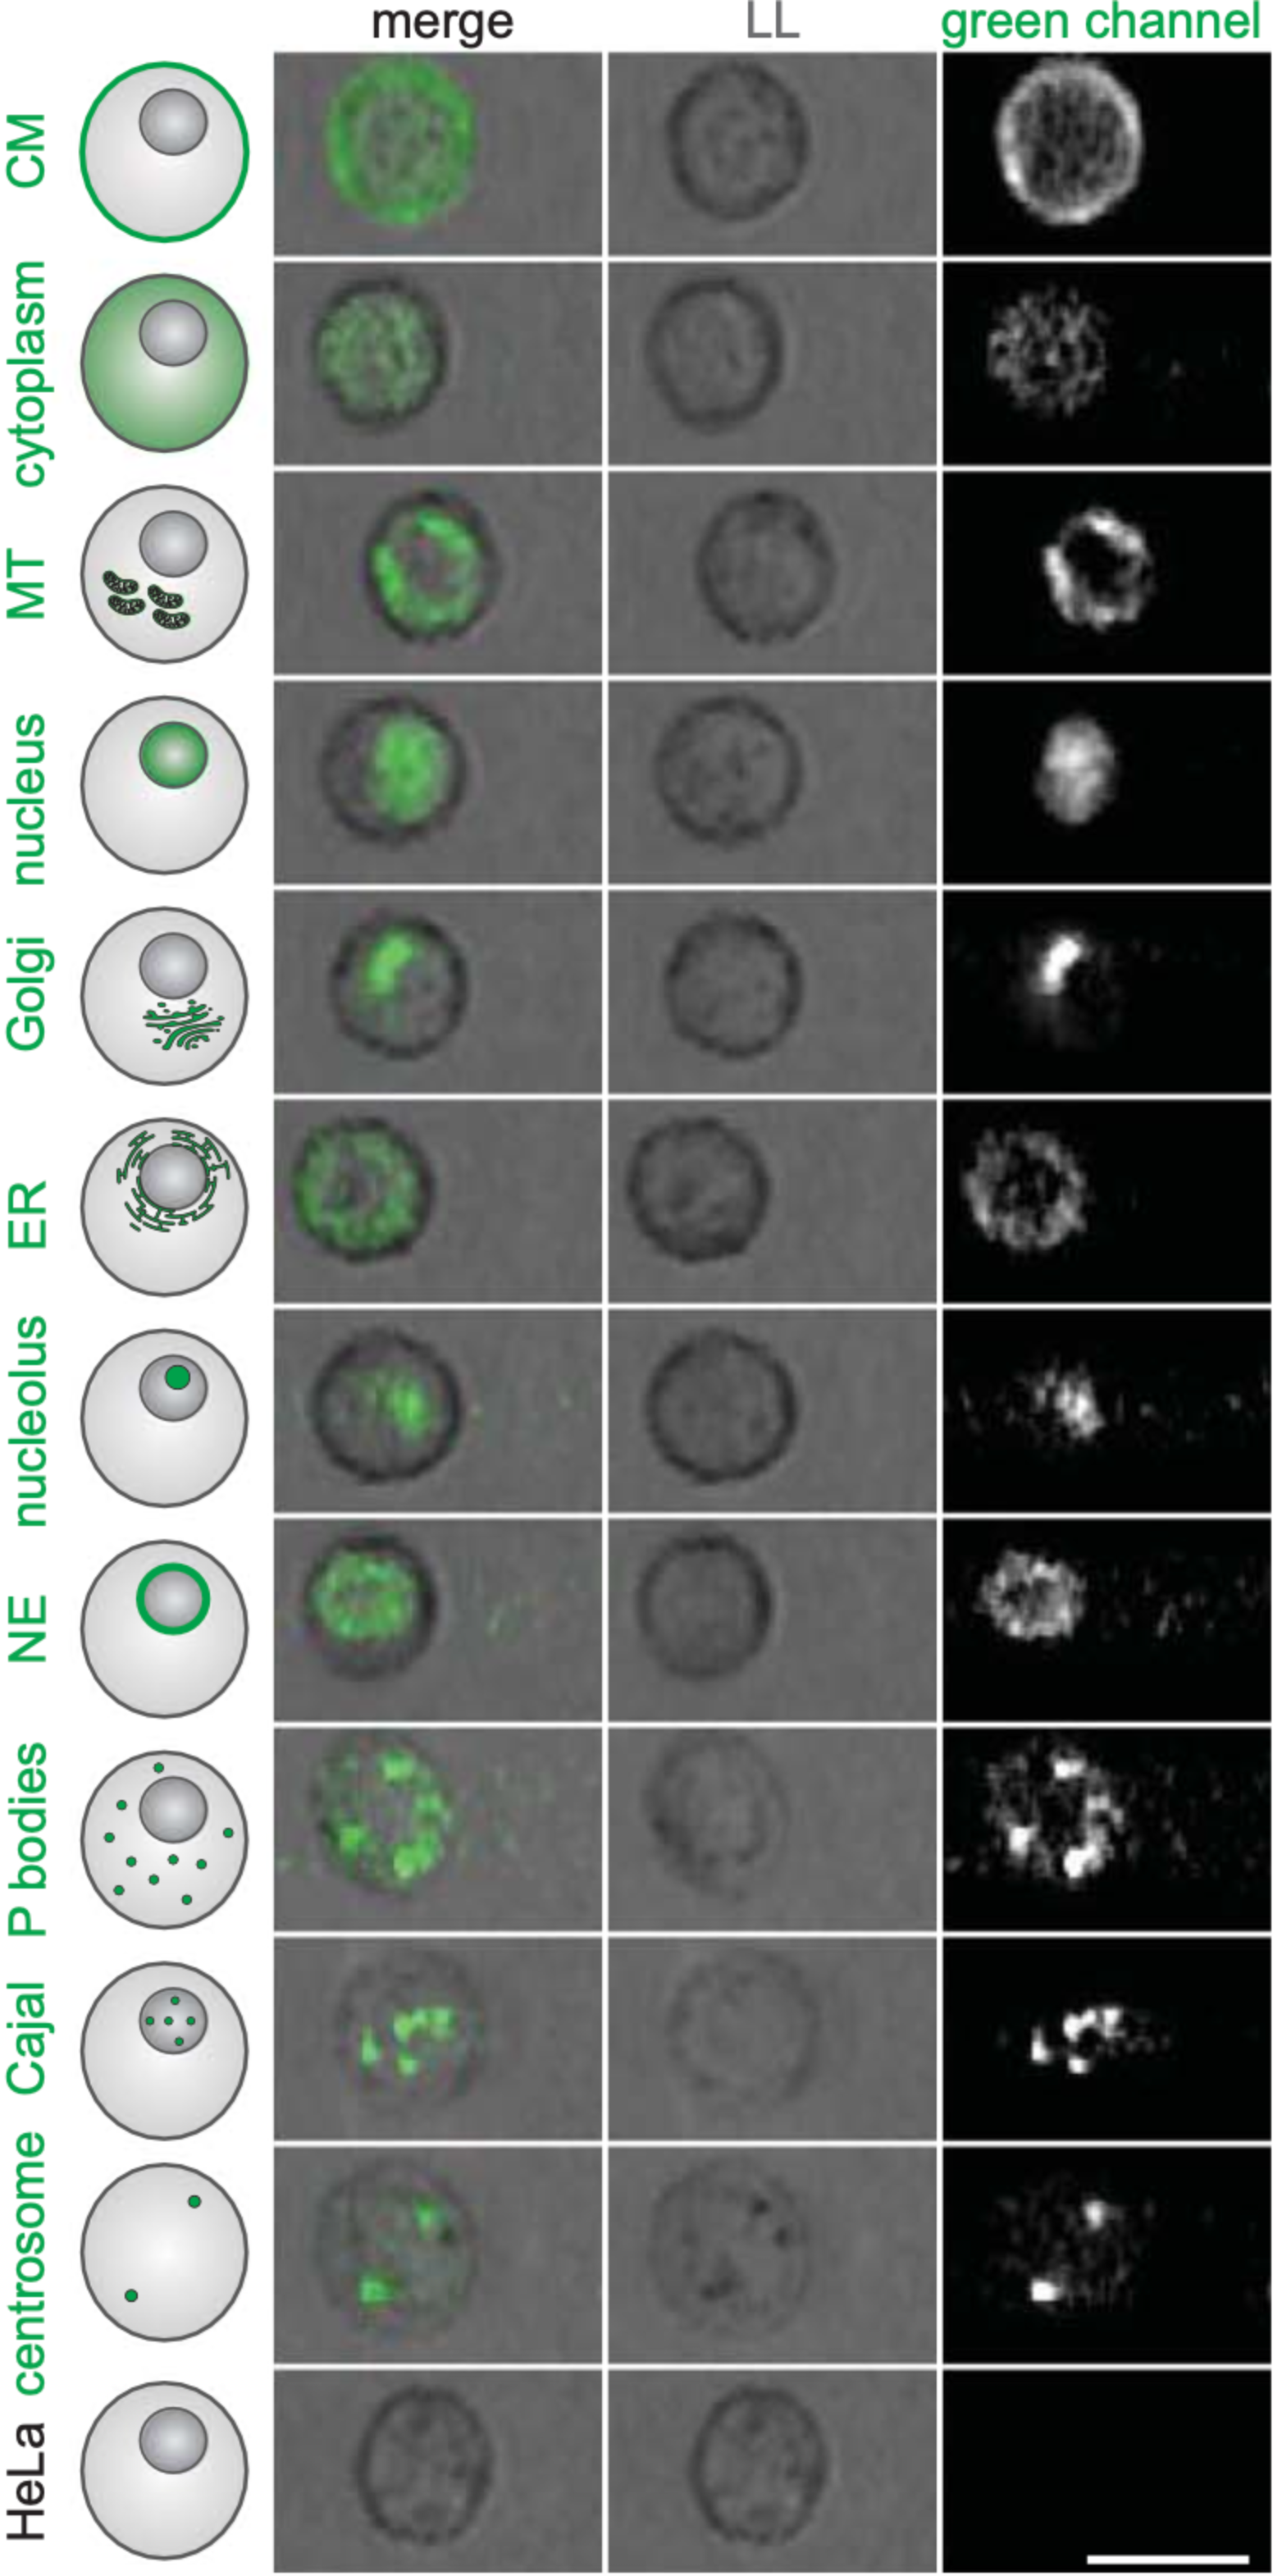
\includegraphics[width=0.5\textwidth]{Figures/ImagingICS.png}
  \caption{ICS-based imaging of HeLa cells expressing fluorescent proteins or stained with specific dyes to target various organelles. Representative images of each organelle are displayed, while the complete datasets comprising 10,000 images each can be accessed as detailed in the data and materials availability section. The following dyes or protein fusions were utilized: cell membrane (Cellmask dye), cytoplasm (GFP fused to HIV Rev nuclear export sequence), mitochondria (Mitotracker dye), nucleus (H2B-mNG), Golgi apparatus (GalNAcT2-GFP), endoplasmic reticulum (ER, ERtracker dye), nucleolus (eGFP-Ki-67), nuclear envelope (LamB1-GFP), P bodies (eGFP-DDX6), Cajal bodies (eGFP-COIL), and centrosomes (anti-pericentrin antibody). P bodies and Cajal bodies were observed in fixed cells, while centrosomes were imaged in fixed and metaphase-stalled cells, resulting in reduced contrast in the light loss (LL) image. Scale bar, 20 mm \cite{doi:10.1126/science.abj3013}.}
  \label{icsimaging}
\end{figure}

\subsection{Unsupervised Machine Learning offers An Automated and Unbiased Approach for Cell Population Profiling}

Cytometry is a common tool used by researchers for profiling cell populations in biological samples. This data can offer insights into the cellular composition of healthy tissues and also reveal how various cell subsets alter under disease conditions. A variety of machine-learning techniques have been developed to annotate known cell populations and to identify new cell subsets from the high-dimensional data generated by cytometry experiments.

Unsupervised machine learning techniques classify cells into groups based on their similarities, as determined solely by cytometry data, without the need for external information. Several generic unsupervised methods can be directly applied to cytometry data. These include popular clustering methods like K-means and hierarchical clustering, probability-based methods like Gaussian mixture models, and density-based methods like HDBSCAN. Unsupervised methods offer several benefits when it comes to enumerating cell populations in high-dimensional space. They allow for an unbiased approach, which is unachievable with manual gating methods, and facilitate the automation of cell population identification with minimal human intervention.


\subsection{Deep Learning-based Embedding for Unsupervised Cell-Type and State Variation Analysis in High-Dimensional Image Data}
In this study, our goal is to develop an embedding that can disentangle complex image features from images that are relevant to cell-type and state variation. This was aimed to be achieved by the application of deep learning to enable biologically meaningful clustering in an unsupervised, unbiased manner in high-dimensional space which can be applied to (multiple) datasets from different experiments.

In addressing the problem at hand, a question arises: do classical image features possess the necessary information to effectively cluster the data into clusters of biological relevance? Should the response be affirmative, the subsequent step involves evaluating the efficiency of the clustering process.

Distance metric learning is a machine learning technique used to learn a distance metric between pairs of data points in a high-dimensional space. The goal of employing distance metric learning in this study is to learn a distance function that accurately reflects the similarity or dissimilarity between the data points, such that similar points are close to each other and dissimilar points are far apart in the learned space. This can be useful for a variety of tasks, such as classification, clustering, and retrieval, where the distance metric plays an important role. Some popular distance metric learning algorithms include large margin nearest neighbor (LMNN), neighborhood component analysis (NCA) and metric learning to rank (MLR). 

If there is not enough information in classical image features to sort classes into clusters of biological relevance, we aimed to proceed to extract complex features from the images, using neural networks leading to clustering based on the latter.

This was targeted to be achieved in two steps. Initially, we utilize pre-trained models in their respective default configurations to evaluate their efficiency in clustering. Next, we identify the top-performing model among those and proceed to fine-tune it by training the same on our data.

\section{Materials \& Methods}
\subsection{Data}
There are three datasets viz. \textit{Salmonella} dataset, Phytoplankton strains dataset and Cell-Cycle dataset. The \textit{Salmonella} dataset contains the images of macrophages infested with \textit{Salmonella}. The idea was to find out what makes the difference between a cell that does not allow bacteria to multiply (n = 1 bacteria per cell), compared to a cell that allows bacteria to multiply (cells with n \> 1 bacteria per cell). Cells are classified on the basis of \textit{Salmonella}(e) present in the cells - One, two and many. The classified images in the \textit{Salmonella} dataset were 655. In phytoplankton dataset, the labelled images were 4304 classified based on the strains. In cell cycle dataset, the annotated images were 17774 based on different mitotic cell cycle stages. Imaging data from the FACSVulcan (ICS) comes in two forms - as numerical values which are included in the exported flow cytometry standard (FCS) file and the actual cell images which are exported as a Z stack of tag image file format (TIFF). Each imaging parameter has 8 numerical values associated with it which correspond to 8 individual TIFFs in the Z stack.

The images are of dimensions - 8 channels (Z-stack), 104 pixels in width, and have variable height ranging from 40 - 90 pixels.

\begin{figure}
  \centering
  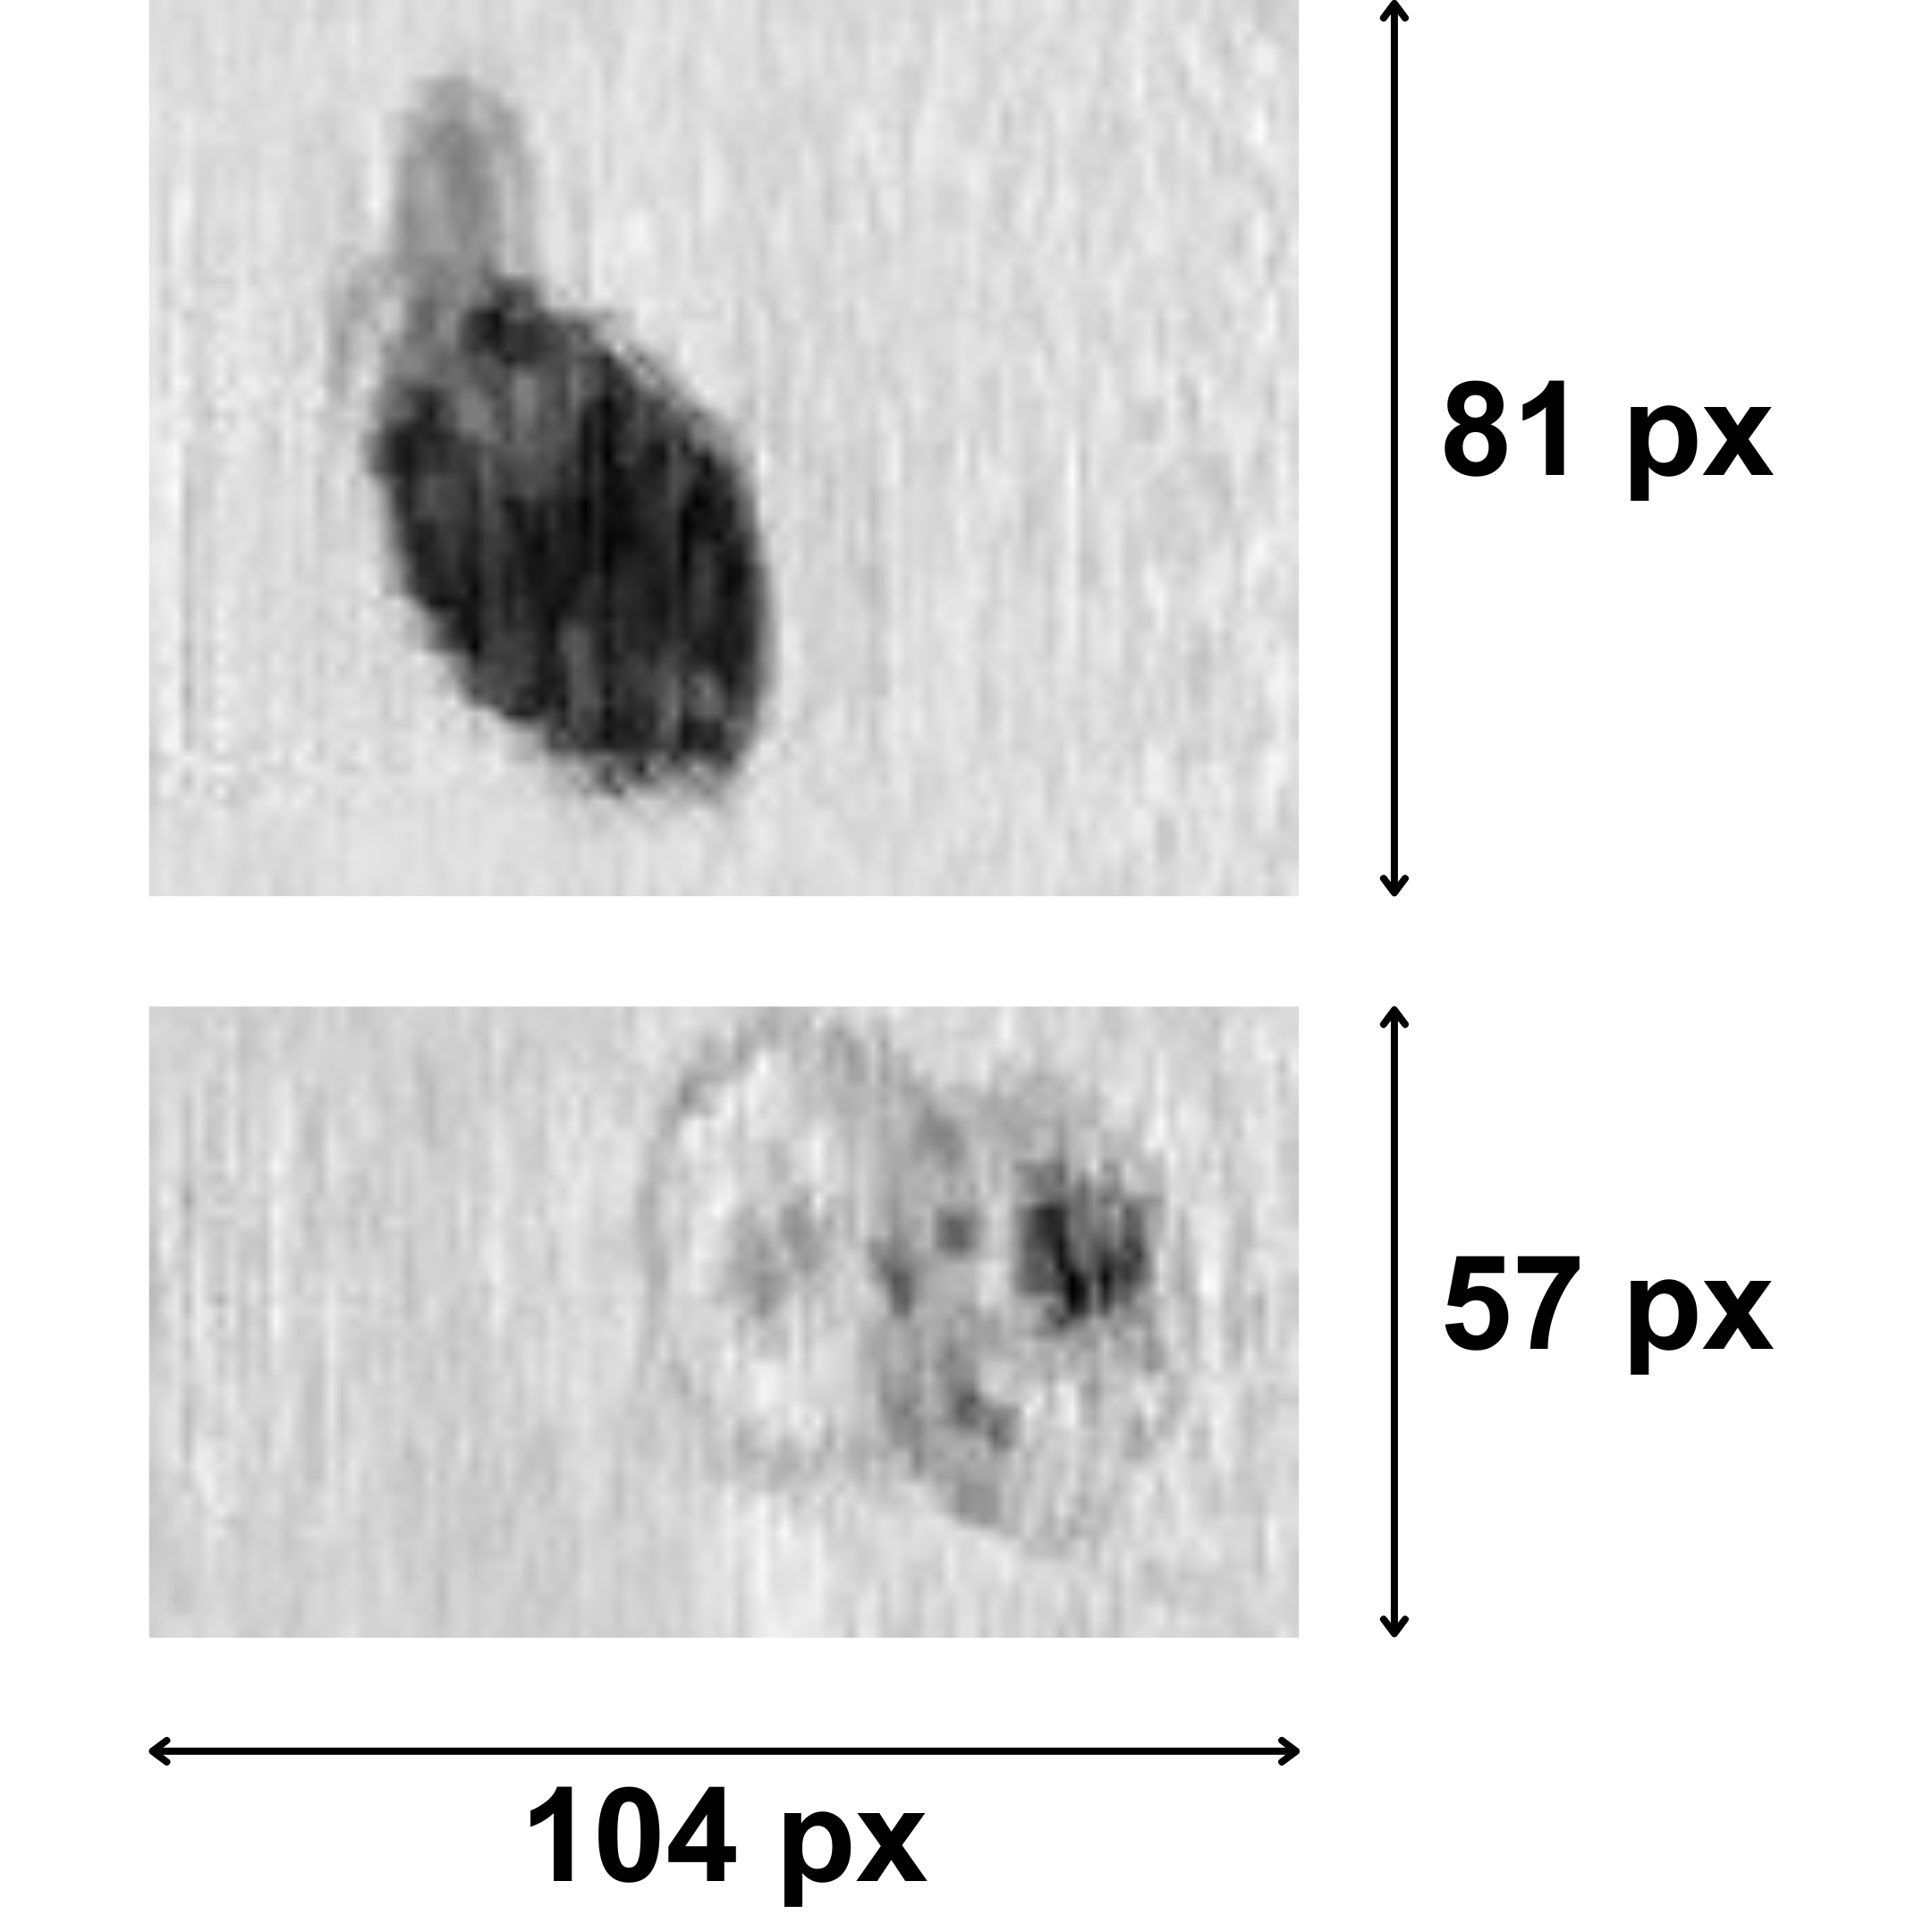
\includegraphics[width=0.5\textwidth]{Figures/sample_img_phytoplankton_cellcycle.png}
  \caption{Random images from the Plankton and Cell Cycle datasets, respectively (Top to Bottom), are displayed in this figure. The image width is fixed at 104 pixels, while the height varies across the images.}
  \label{sampleimgs}
\end{figure}

\subsection{Data Format for Classical Image features for Data Analysis, Processing}
\label{adata_scanpy}
For the analysis, processing of classical image features, the data output file .csv, was made into an AnnData object. AnnData.X contained the features as an observations x variations data matrix, the names of the features in AnnData.var as one-direction variables annotation, and the metadata in AnnData.obs as one-direction observations annotations.

Anndata is a data format and a python package for handling annotated data matrices, positioned between pandas and xarray \cite{virshup_rybakov_theis_angerer_wolf_2021}. Multidimensional annotations are stored in obsm and varm. Unstructured data which doesn’t fit the model, but should stay associated with the dataset are stored in uns. Principal components and the transformed dimensionality-reduced data matrix obtained through PCA can be stored as multi-dimensional annotations of variables and observations respectively (in obsm and varm) \cite{virshup_rybakov_theis_angerer_wolf_2021}.

\begin{figure}
  \centering
  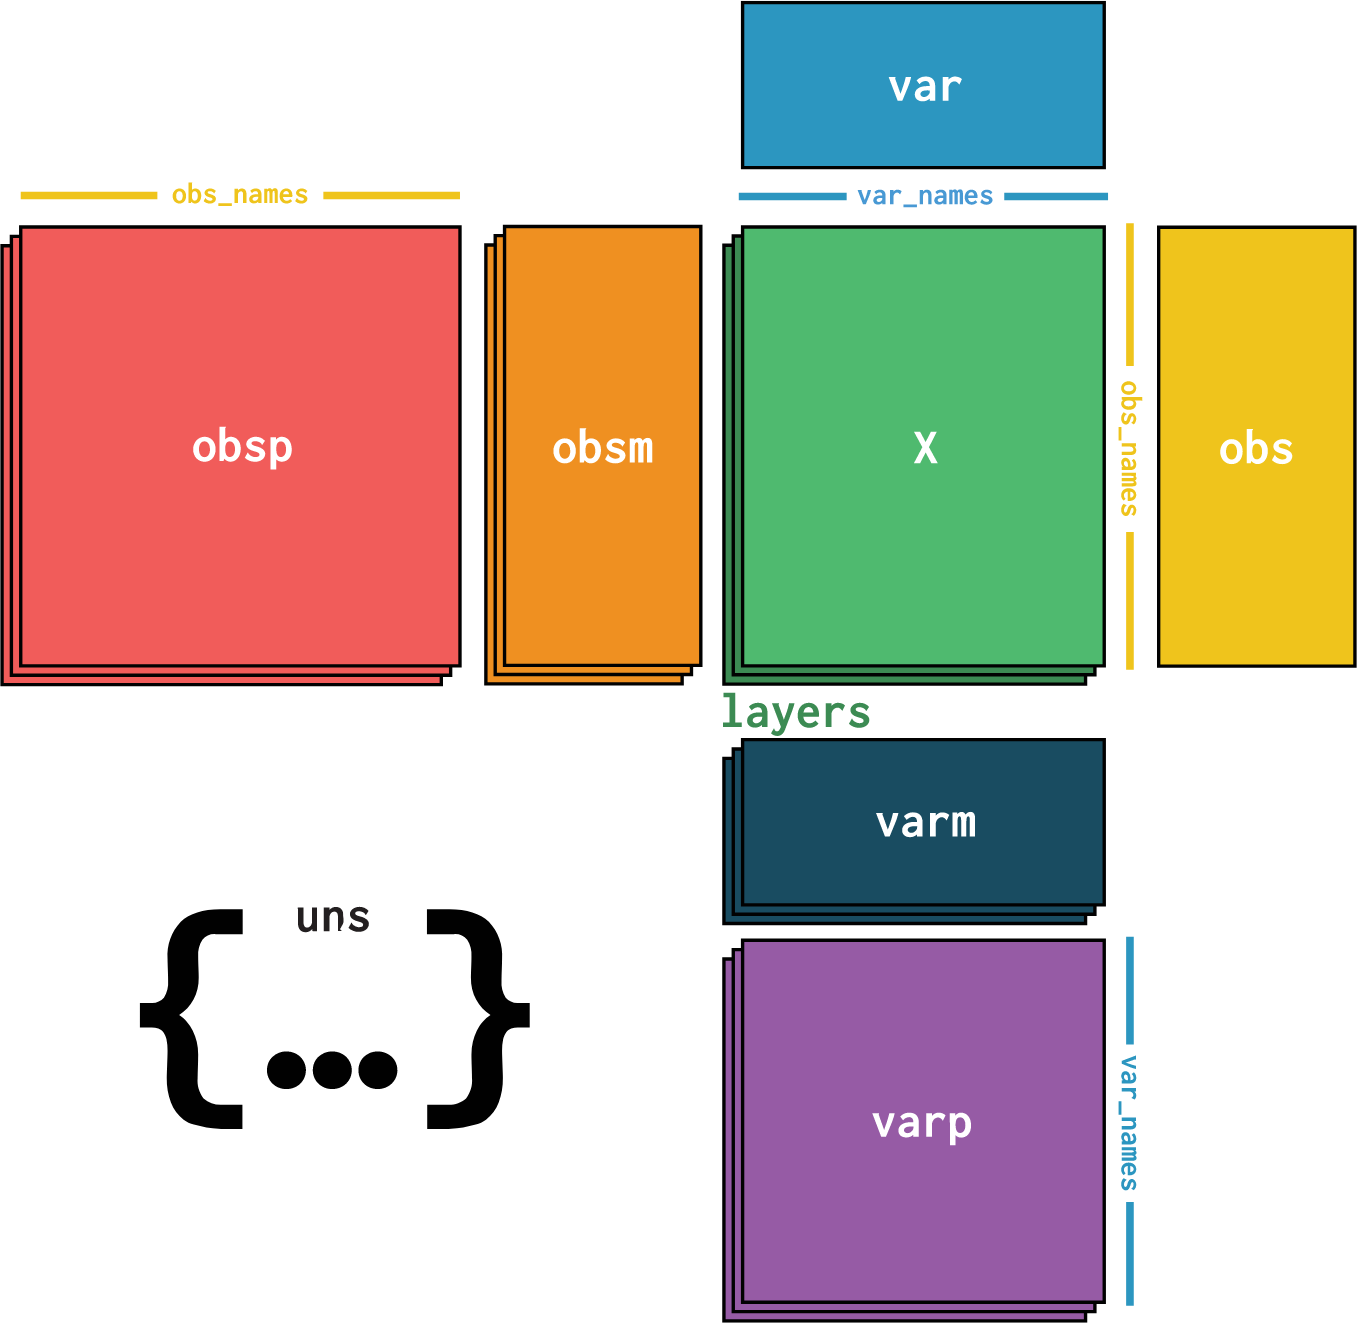
\includegraphics[width=0.7\textwidth]{Figures/anndata_schema.png}
  \caption{AnnData schema, a data structure used in single-cell genomics, combines a data matrix X with annotations of observations (obs), variables (var), and unstructured annotations (uns). The obs component contains information about individual cells or samples, while the var component stores details about variables, typically genes. Additionally, the obsm and varm components can accommodate multi-dimensional observations or variables, respectively. The obsp and varp components allow for the storage of pairwise observations or variables, such as distances or correlations. The uns component provides a flexible container for any additional annotations or metadata. Together, these components within the AnnData format provide a comprehensive and standardized framework for organizing and analyzing single-cell data.}
  \label{adata}
\end{figure}

The data was processed and analyzed using the tools and methods provided by the Scanpy package, an open-source Python library for single-cell RNA sequencing (scRNA-seq) data analysis \cite{wolf_angerer_theis_2018}. Scanpy offers a comprehensive set of functionalities for quality control, preprocessing, visualization, and downstream analysis of scRNA-seq data. It implements various algorithms and approaches for tasks such as dimensionality reduction, clustering, trajectory inference, and differential expression analysis \cite{wolf_angerer_theis_2018}.

\subsection{Pre-trained Models}
We selected the neural network models ResNET50, ScDINO, TransPath out-of-the box to analyse how the models perform in forming meaningful clusters. The best performing network is selected for fine-tuning on the available datasets.

To fit our images to the models, to extract features, the images were padded with zeros to fit the dimensions of the images. The images were processed in a channel-wise manner, with similar calculations applied to each channel.

\subsubsection{ResNet50}
ResNET50, part of Residual Network (ResNet) family, is a deep convolutional neural network architecture having 50 layers which is used for image recognition and classification tasks \cite{DBLP:journals/corr/HeZRS15}. ResNet50 was trained on ImageNet dataset - over 14 million images that are organized into more than 20,000 categories. The network was trained on images of dimensions 224x224, RGB \cite{DBLP:journals/corr/HeZRS15}. The images were pre-processed before they were used to train the model. This preprocessing included resizing the images to 224x224 pixels, subtracting the mean RGB values from the images, and normalizing the images. ResNet50 is commonly employed as a pre-trained model for transfer learning, where the model is pre-trained on a large dataset, such as ImageNet, and then fine-tuned for a specific classification task with a smaller dataset. By leveraging the learned features from the pre-trained model, transfer learning often leads to better performance compared to training a model from scratch, particularly when the available training data is limited. The loss function of ResNet50 depends on the specific task it is being used for \cite{DBLP:journals/corr/HeZRS15}. However, in the case of image classification, the typical loss function used with ResNet50 is the softmax cross-entropy loss. Given an input image, the ResNet50 network predicts the probabilities of each class using the softmax activation function in the last layer. The softmax function normalizes the output logits into probabilities, representing the network's confidence for each class. The softmax cross-entropy loss measures the discrepancy between the predicted class probabilities and the true labels. It encourages the network to assign higher probabilities to the correct class and lower probabilities to the incorrect classes. The loss function is computed as the average of the cross-entropy losses over all the training samples. Mathematically, the softmax cross-entropy loss for ResNet50 can be defined as:

\[
\mathcal{L} = -\frac{1}{N}\sum_{i=1}^{N}\sum_{j=1}^{C}y_{ij}\log(p_{ij})
\]

Where:
\begin{itemize}
\item $\mathcal{L}$ is the loss function,
\item $N$ is the number of training samples,
\item $C$ is the number of classes,
\item $y_{ij}$ is the true label (1 if the sample belongs to class $j$, 0 otherwise),
\item $p_{ij}$ is the predicted probability for class $j$ for the $i$-th sample \cite{DBLP:journals/corr/HeZRS15}.
\end{itemize}

\paragraph{} Working of ResNet50: ResNet's primary innovation is the use of residual connections, also known as skip connections or shortcut connections, which enable the network to overcome the vanishing gradient problem and facilitate the training of much deeper networks \cite{DBLP:journals/corr/HeZRS15}. The vanishing gradient problem arises when gradients become too small during the backpropagation process, making it difficult for the network to learn and update weights effectively \cite{DBLP:journals/corr/HeZRS15}.Residual connections work by allowing the output of one layer to be added to the output of a layer further down the network. This means that the network essentially learns the residual function (i.e., the difference between the input and output of a series of layers), rather than the direct mapping between input and output \cite{DBLP:journals/corr/HeZRS15}. This approach helps maintain gradient flow through the network, resulting in improved training performance and better convergence \cite{DBLP:journals/corr/HeZRS15}.

\subsubsection{scDINO}
Single Cell Distillation of knowledge with No labels is the application of DINO model for automated microscopy-derived fluorescent imaging datasets of single cells \cite{Pfaendler2023.01.16.524226}. DINO is a self-supervised vision transformer capable of learning representations from unlabelled data using a contrastive loss function \cite{Pfaendler2023.01.16.524226}. The model consists of a student ViT (Vision Transformer) that learns to predict global features in an image from local patches, supervised by the cross-entropy loss from a momentum teacher ViT's embeddings while doing centering and sharpening to prevent mode collapse \cite{Pfaendler2023.01.16.524226}. The DINO model is able to automatically learn class-specific features leading to accurate unsupervised object segmentation \cite{Pfaendler2023.01.16.524226}. The loss function used in the DINO model is a contrastive loss function that is applied to all views at once, and the goal of backpropagation is to minimize the cross-entropy loss between the student and teacher models. The loss function of the DINO model is a cross-entropy loss function applied to all views at once \cite{Pfaendler2023.01.16.524226}.

\begin{figure}
  \centering
  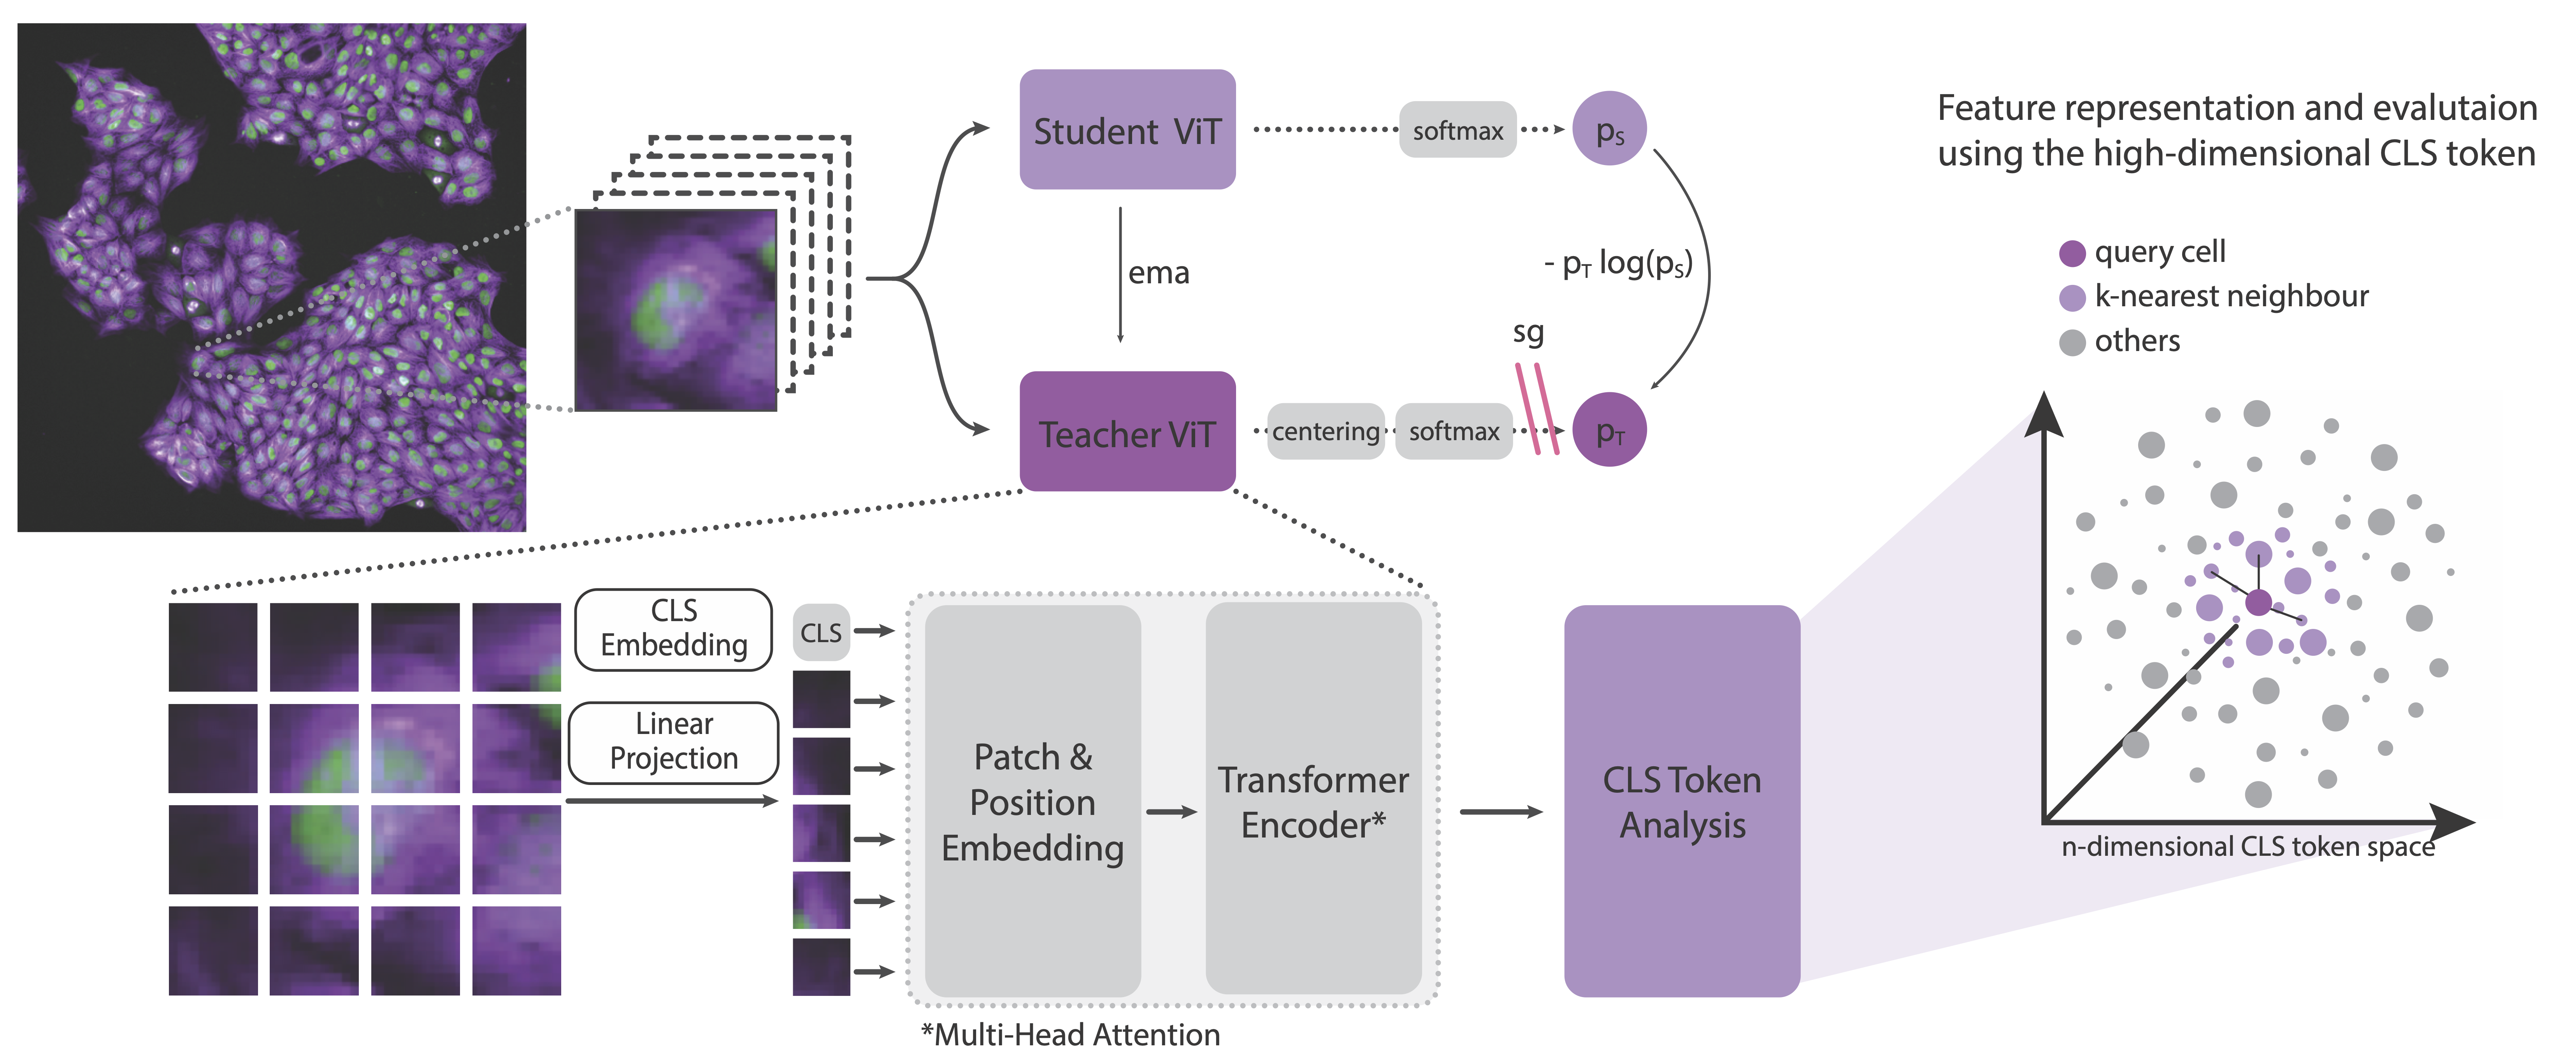
\includegraphics[width=\textwidth]{Figures/scDINO_working.png}
  \caption{Workflow for single-cell phenotyping using DINO-based self-supervised vision transformers (ss-ViTs). The upper part illustrates the DINO-based self-supervised learning approach, which includes a student and teacher ViT. The lower part showcases the ViT-based image embedding and feature representations, with emphasis on the CLS token, utilized for single-cell clustering \cite{Pfaendler2023.01.16.524226}.}
  \label{scdinoworking}
\end{figure}

$$
L(\theta) = -\frac{1}{N} \sum_{i=1}^{N} \sum_{v=1}^{V} \log \frac{e^{\frac{z_{i,v}^s \cdot z_{i,v}^t}{\tau}}}{\sum_{j=1}^{N} e^{\frac{z_{i,v}^s \cdot z_{j,v}^t}{\tau}}}
$$

Where:
\begin{itemize}
\item $L(\theta)$: Loss function
\item $N$: Number of samples
\item $V$: Number of views
\item $z_{i,v}^s$: Student embedding for the $i$-th sample and $v$-th view
\item $z_{i,v}^t$: Teacher embedding for the $i$-th sample and $v$-th view
\item $\tau$: Temperature scaling factor
\end{itemize}

The goal of the DINO model is to minimize this loss function, which encourages the student model to learn representations that are similar to the teacher model. The temperature scaling factor $\tau$ controls the sharpness of the probability distribution over the embeddings \cite{Pfaendler2023.01.16.524226}.

scDINO was adapted to accept variable numbers of input channels and averaged the RGB-specific embedding weights, giving each channel equal weight \cite{Pfaendler2023.01.16.524226}. scDINO was trained on 89,564 cells in the immune single-cell training dataset, while using 224x224x5 as input data. All the pixel intensities were rescaled to range between 0 and 1 for each channel \cite{Pfaendler2023.01.16.524226}.

\subsubsection{TransPath}
TransPath is a transformer based unsupervised contrastive learning model for histopathological image classification. TransPath is a hybrid model that combines a convolutional neural network (CNN) with a swin-transformer architecture \cite{WANG2022102559}. The CNN is used to extract local features from the images, while the transformer is used to learn long-range dependencies between the features \cite{WANG2022102559}. This allows TransPath to learn both local and global features from the images, which is important for histopathological image classification. TransPath was trained on a dataset of histopathological images that were labeled with the type of cancer. The model was trained using a self-supervised learning method called contrastive learning. Contrastive learning involves learning to distinguish between similar and dissimilar images \cite{WANG2022102559}. This allows TransPath to learn to identify subtle differences in histopathological images, which is important for cancer classification. The model was trained on histopathological images of dimensions 224 x 224 x 3. TransPath has been shown to achieve state-of-the-art performance on the task of histopathological image classification. It has been shown to be able to classify different types of cancer with high accuracy \cite{WANG2022102559}. The loss function is the similar to the DINO - contrastive loss with cross-entropy:

% \[
% L = -\sum_{i=1}^{N} \log \left( \frac{e^{\frac{q_{i} \cdot k_{i}}{\tau}}}{\sum_{j=1}^{N} e^{\frac{q_{i} \cdot k_{j}}{\tau}}} \right) - \sum_{i=1}^{N} \log \left( \frac{e^{\frac{k_{i} \cdot q_{i}}{\tau}}}{\sum_{j=1}^{N} e^{\frac{k_{i} \cdot q_{j}}{\tau}}} \right) + \lambda \cdot \text{CELoss}(q, y)
% \]
\[
L = -\sum_{i=1}^{N} \log \left( \frac{e^{\frac{q_{i} \cdot k_{i}}{\tau}}}{\sum_{j=1}^{N} e^{\frac{q_{i} \cdot k_{j}}{\tau}}} \right) - \sum_{i=1}^{N} \log \left( \frac{e^{\frac{k_{i} \cdot q_{i}}{\tau}}}{\sum_{j=1}^{N} e^{\frac{k_{i} \cdot q_{j}}{\tau}}} \right) + \lambda \cdot \mathrm{CELoss}(q, y)
\]

In this formula:
\begin{itemize}
\item \(N\) represents the total number of instances or samples.
\item \(q_i\) and \(k_i\) are the query and key embeddings, respectively, for instance \(i\).
\item \(\tau\) denotes the temperature hyperparameter that controls the similarity scaling.
% \(\text{CELoss}(q, y)\) refers to the cross-entropy loss between the predicted logits \(q\) and the true labels \(y\).
\item \(\text{CELoss}(q, y)\) refers to the cross-entropy loss between the predicted logits \(q\) and the true labels \(y\).
\item \(\lambda\) represents the weighting factor for the cross-entropy loss.
\end{itemize}

This loss function encourages the query and key embeddings to form positive pairs (similar instances) while discouraging negative pairs (dissimilar instances) based on their similarities measured using the dot product. Additionally, the cross-entropy loss term ensures the model's predictions align with the true labels.

\subsection{Cluster Purity Evaluates the Performance of Biologically Meaningful Cluster Formation}
\label{cp}

Cluster purity was developed to quantitatively measure the cluster separation. Purity provides a simple and transparent evaluation of clustering quality. It is computed by assigning each cluster to the class that is most frequent within the cluster and then measuring the accuracy of this assignment by counting the number of correctly assigned documents \cite{ISBN_0521865719}. Purity values range between 0 and 1, where higher values indicate better clustering quality \cite{ISBN_0521865719}. This is calculated using the formula:
$$
Purity = \frac{1}{N} \sum_{i=1}^{k} \max_j |c_i \cap t_j|
$$
where
\begin{itemize}
	\item $N$ is the number of objects (data points),
	\item $k$ is the number of clusters,
	\item $c_i$ represents a cluster in $C$, and
	\item $t_j$ is the classification which has the maximum count for cluster $c_i$.
\end{itemize}

In our case, to calculate Purity, the following steps are followed. Firstly, a confusion matrix is created, which involves counting the number of objects classified as each class within each cluster. This matrix helps determine the overlap between the assigned clusters and the ground truth classifications.

Next, for each cluster, the maximum value in its corresponding row of the confusion matrix is selected. These maximum values represent the highest number of correct classifications achieved within each cluster. Finally, these maximum values are summed together, and the resulting sum is divided by the total number of data points.

\section{Results}
\subsection{Classical image features are inadequate for forming biologically meaningful clusters}
Across the two datasets - \textit{Salmonella} and Phytoplankton, the classical images features were extracted and plotted in histograms. After the pre-processing of data by normalization and scaling, PCA (principle component analysis, used for dimensionality reduction to simplify datasets with large number of variables) was performed using scanpy functions \ref{adata_scanpy}, \cite{pca}. Then, UMAP (Uniform Manifold Approximation and Projection (UMAP) is a dimensionality reduction technique that is often used in the field of machine learning and data science \cite{umap}. UMAP is used to reduce the dimensionality of data, but it does so in a way that preserves much more of the data's structure \cite{umap}, particularly the relationships between points) was performed using ScanPy functions \ref{adata_scanpy}.

\begin{figure}
  \centering
  \begin{subfigure}{\linewidth}
    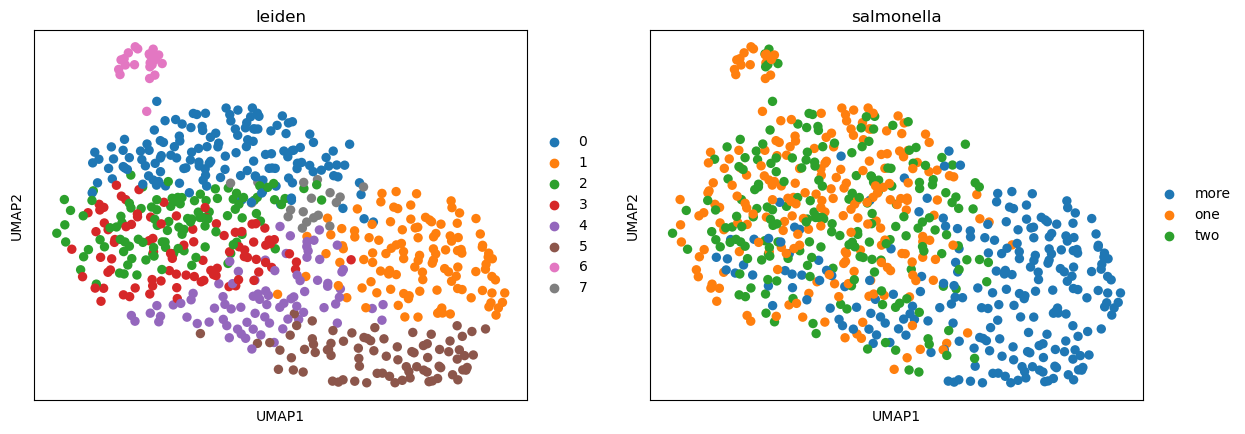
\includegraphics[width=\linewidth]{Figures/salmonella_clusters_before_DML.png}
    \caption{Leiden clustering of Salmonella data. This visualization represents the distinct clusters identified in the Salmonella dataset following the pre-processing stage.}
    \label{multifig1:image_a}
  \end{subfigure}
  \hfill
  \begin{subfigure}{\linewidth}
    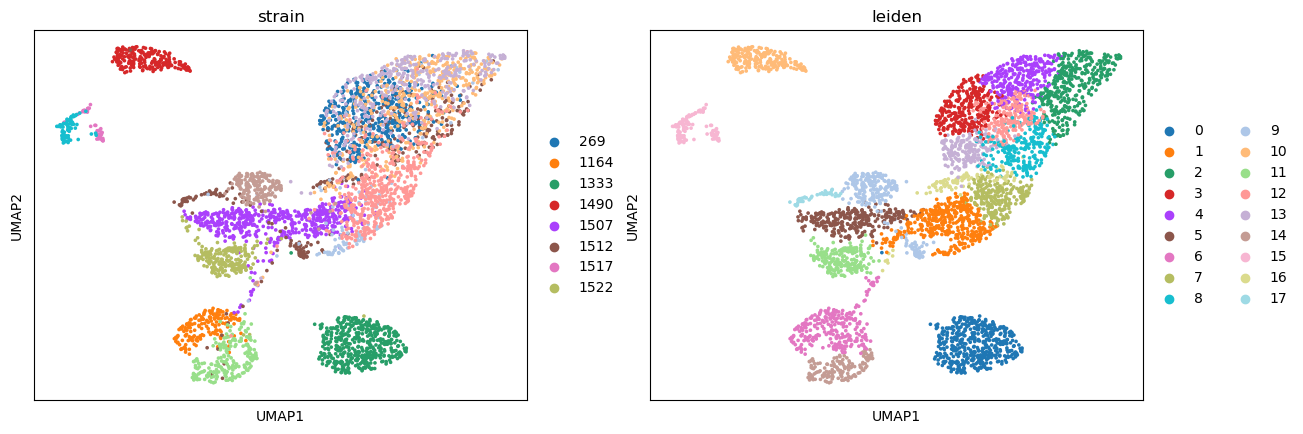
\includegraphics[width =\linewidth]{Figures/plankton_clusters_before_DML.png}
    \caption{Leiden clustering of Plankton data. This diagram illustrates the various clusters discerned in the Plankton dataset after the pre-processing phase.}
    \label{multifig1:image_b}
  \end{subfigure}
  \hfill
  \begin{subfigure}{\linewidth}
    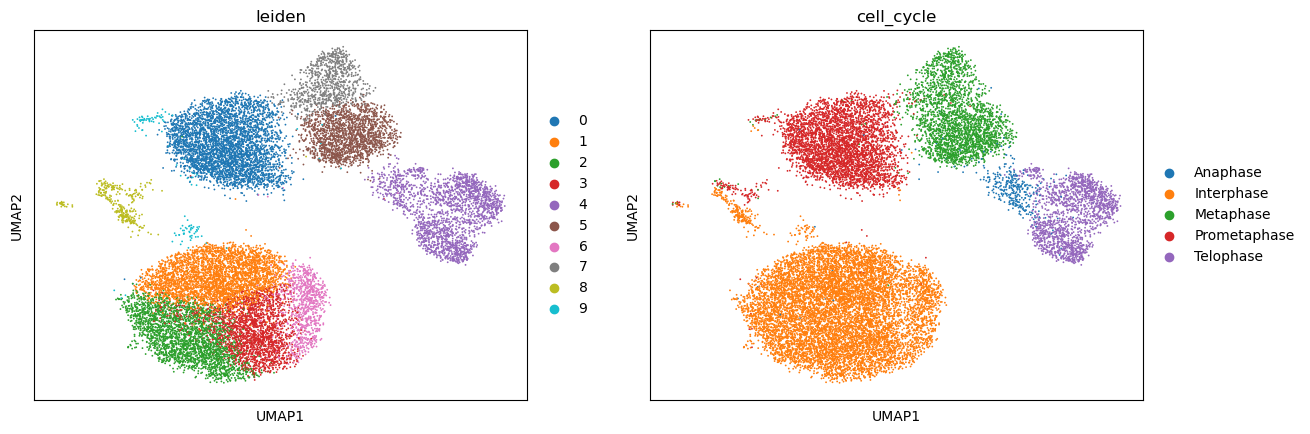
\includegraphics[width=\linewidth]{Figures/cellcycle_clusters_before_DML.png}
    \caption{Leiden clustering of Cell Cycle data. This image depicts the unique clusters found in the Cell Cycle dataset post the pre-processing step.}
    \label{multifig1:image_c}
  \end{subfigure}
  \caption{Each figure provides a visual representation of the data clustering, aiding in the biological interpretation of each distinct group.}
  \label{multifig1:overall_figure}
\end{figure}


It is to be noted that some clusters, strains could not be distinctly separated in the initial stages of this process.

\subsection{Limited performance of scaling in embedding}
The objective of feature scaling is to establish an equal contribution from all features to the predictive model, thereby preventing the undue influence of features with larger values. This becomes particularly crucial when dealing with datasets that encompass features with dissimilar ranges, units of measurement, or magnitudes. The implementation of feature scaling allows for the transformation of the dataset’s features onto a more uniform scale, thereby enhancing the efficacy. By ensuring a balanced comparison between features, scaling not only improves model convergence but also mitigates the risk of certain features dominating others based purely on their magnitude.

However, upon the scaling and transformation of the feature space, a clear demarcation between the strains becomes evident, as illustrated in \ref{clustersafterscaling}. The transformation process involves the scaling of features after subsetting the dataset, a step that amplifies the subtle differences in features across various classes. The basis for these transformations lies in the weighted Euclidean distances between data points in the feature space (\ref{multifig2:overall_figure}). This amplification, facilitates the separation of the clusters. By magnifying the differences, we are able to discern clear boundaries between clusters that might otherwise appear to overlap or blend into each other. The clusters, 269, 1164, 1333, 3015, 3541 are used to illustrate the effect of transformation of feature space and scaling on cluster separation.

\begin{figure}
  \centering
  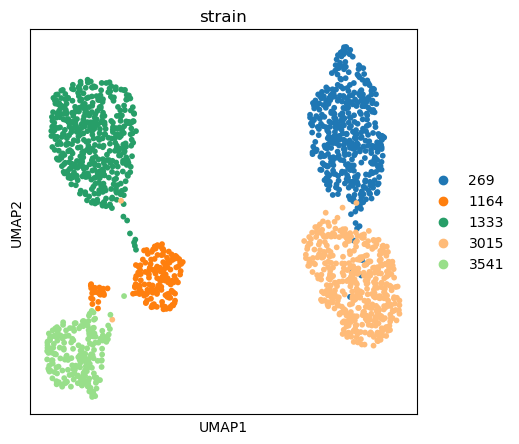
\includegraphics[width=0.45\textwidth]{Figures/phytoplanktonclusterseparationafterscaling.png}
  \caption{The image illustrates the distinct separation of phytoplankton strain clusters 269, 1164, 1333, 3015, 3541, a result of the applied scaling procedure. This clear demarcation contrasts with the initial state where these clusters were not clearly separated, as depicted in \ref{multifig1:image_b}. The scaling procedure has thus significantly enhanced the clarity and differentiation of these phytoplankton strain clusters.}
  \label{clustersafterscaling}
\end{figure}

\begin{figure}
  \centering
  \begin{subfigure}{0.45\linewidth}
    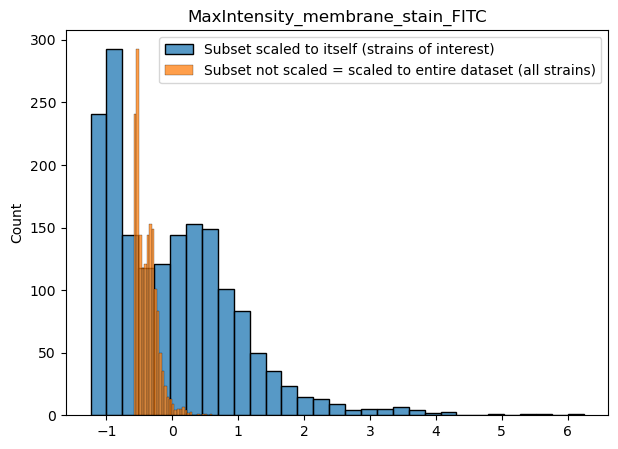
\includegraphics[width=\linewidth]{Figures/maxintensitymembranestain_fitc_scaledandunscaled_planktondata.png}
    \caption{Histogram comparing the distribution of the maximum intensity of membrane stain FITC in two different subsets of data.}
    \label{multifig2:image_a}
  \end{subfigure}
  \hfill
  \begin{subfigure}{0.4\linewidth}
    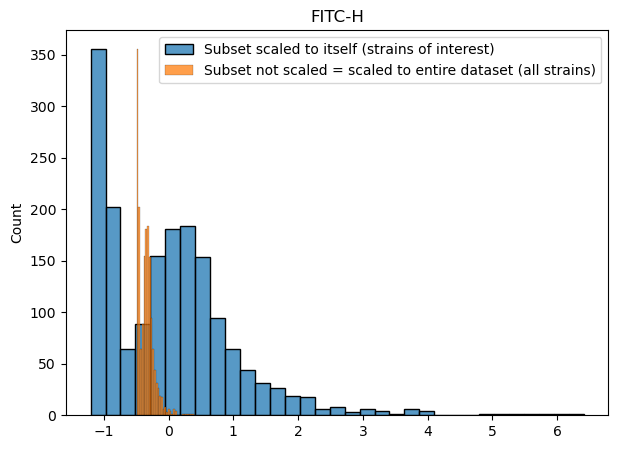
\includegraphics[width=\linewidth]{Figures/fitc-h_scaledandunscaled_planktondata.png}
    \caption{Histogram that compares the intensity of the stain FITC-H in two different data.}
    \label{multifig2:image_b}
  \end{subfigure}
  \caption{Each figure depicts how the differences across the clusters are amplified upon scaling, in comparison to the unscaled. Each figure represents a classical feature selected - MaxIntensity\_membrane\_stain\_FITC and FITC-H among the selected plankton strains - 4281, 3003, 1512, referred in the images as strains of interest.}
  \label{multifig2:overall_figure}
\end{figure}

Despite the transformation of feature space, some clusters could not be clearly distinguished from each other as shown in \ref{multifig3:overall_figure} - depicts the clusters of one salmonella and two salmonellae not being able to be separated from each other, yet after scaling and the transformation of the feature space. Moreover, similar trend is observed when trying to separate the phytoplankton strains - 1512, 3003 and 4281.

\begin{figure}
  \centering
  \begin{subfigure}{0.5\linewidth}
    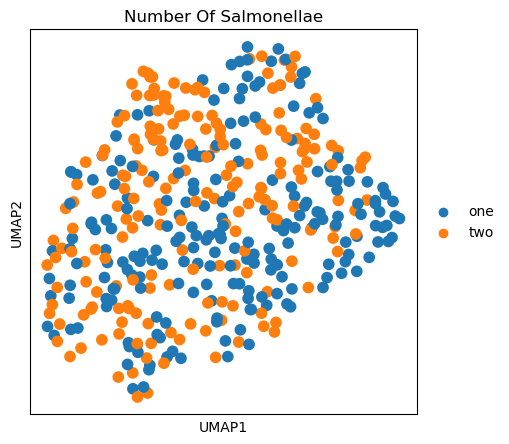
\includegraphics[width=\linewidth]{Figures/clustersmixedafterscalingsalmonella.png}
    \caption{Depicts the \textit{Salmonella} clusters one and two, demonstrating their lack of clear separation despite undergoing scaling and transformation.}
    \label{multifig3:image_a}
  \end{subfigure}
  \hfill
  \begin{subfigure}{0.5\linewidth}
    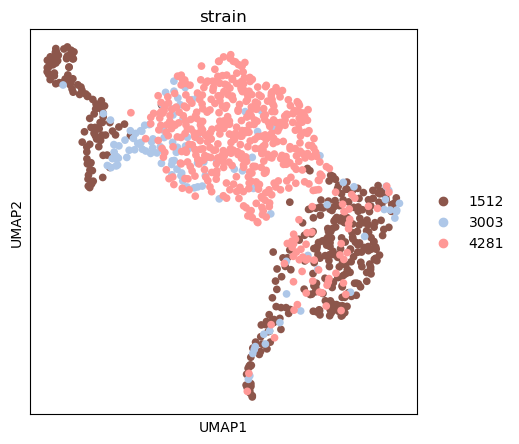
\includegraphics[width=\linewidth]{Figures/clustersmixedafterscalingplankton.png}
    \caption{Illustrates the plankton clusters of strains 1512, 3003, and 4281, emphasizing their continued overlap even after scaling and transformation.}
    \label{multifig3:image_b}
  \end{subfigure}
  \caption{Illustration of the two datasets' clusters post scaling and feature space transformation, highlighting the lack of clear separation between them.}
  \label{multifig3:overall_figure}
\end{figure}


\subsection{Insufficient Separation of Biologically Meaningful Clusters Using Distance Metric Learning on Classical Image Features}

To ascertain the feature space that facilitates the formation (and separation) of biologically relevant clusters, we implemented the application of distance metric learning. Distance metric learning was performed on the classical image features. The distance metric learning algorithms used include: Neighborhood Component Analysis (NCA), Large Margin Nearest Neighbors (LMNN), Metric Learning for Kernel Regression (MLKR) and Local Fischer Discriminant Analysis  for Supervised Dimensionality Reduction (LFDA).

\textbf{NCA:} Through supervised learning, it learns a linear transformation with the aim of boosting the precision of a stochastic nearest neighbors rule within the transformed space.

\textbf{LMNN:} acquires a Mahalanobis distance metric within the context of kNN classification. The metric it learns tries to maintain proximity among k-nearest neighbors belonging to the same class, while ensuring a large margin instances from different classes. Importantly, this algorithm operates without making presumptions about the distribution of the data.

\textbf{MLKR:} This function learns distance function by minimizing the leave-one-out regression error. This can also be used for dimensionality reduction and high dimensional data visualization.

\textbf{LFDA:} It is beneficial in situations of multimodality, where one or multiple classes form distinct clusters within the input space.

Distance metric learning was performed after the dimensionality reduction was executed on the dataset using PCA \cite{pca}.

Out of the aforementioned distance metric learning algorithms, NCA was the best-performing algorithm based on the results from cluster purity calculation - \ref{tab:performanceofDML}.


\begin{table}[h]
\small
\centering
\caption{Performance of different distance metric learning algorithms across multiple datasets. The performance was measured using the cluster purity metric mentioned in \ref{cp}.}
\label{tab:performanceofDML}
\begin{tabular}{lccc}
\hline
\textbf{Distance Metric} & \textbf{Salmonella} & \textbf{Phytoplankton} & \textbf{Cell Cycle} \\
\hline
No\_DistanceMetricLearning & 0.568433 & 0.673014 & 0.852585 \\
NCA & 0.72579 & 0.76682 & 0.99339 \\
LMNN & 0.63115 & 0.67778 & 0.99325 \\
MLKR & 0.69221 & 0.76703 & 0.99182 \\
LFDA & 0.56843 & 0.72847 & 0.87293 \\
\hline
\end{tabular}
\end{table}

% \begin{table}[h]
% \centering
% \caption{Performance of different distance metric learning algorithms across multiple datasets. The performance was measured using the cluster purity metric mentioned in \ref{cp}.}
% \begin{tabularx}{\textwidth}{|X|X|X|X|}
% \hline
% \textbf{Distance Metric Learning Algorithm} & \textbf{Salmonella Dataset} & \textbf{Phytoplankton Dataset} & \textbf{Cell Cycle Dataset} \\
% \hline
% \textbf{No\_DistanceMetricLearning} & 0.568433 & 0.673014 & 0.852585 \\
% \textbf{NCA} & 0.72579 & 0.76682 & 0.99339 \\
% \textbf{LMNN} & 0.63115 & 0.67778 & 0.99325 \\
% \textbf{MLKR} & 0.69221 & 0.76703 & 0.99182 \\
% \textbf{LFDA} & 0.56843 & 0.72847 & 0.87293 \\
% \hline
% \end{tabularx}
% \label{tab:performanceofDML}
% \end{table}


The cluster purity increased noticably. Some clusters couldn't be separated despite the application of distance metric learning as observed in \ref{multifig4:DML_Clusters}.

\begin{figure}
  \centering
  \begin{subfigure}{\linewidth}
    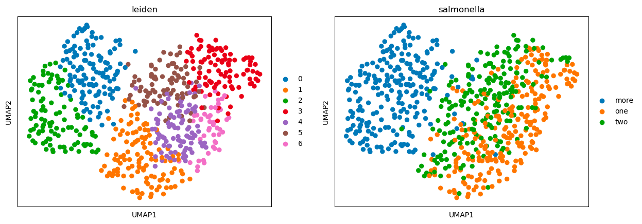
\includegraphics[width=\linewidth]{Figures/salmonellaclustering_afternca.png}
    \caption{Leiden clustering of \textit{Salmonella} data after the application of distance metric learning algorithm NCA.}
    \label{multifig4:image_a}
  \end{subfigure}
  \hfill
  \begin{subfigure}{\linewidth}
    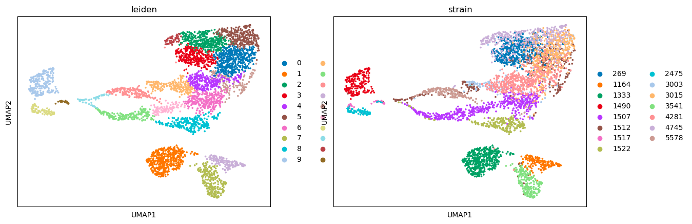
\includegraphics[width=\linewidth]{Figures/planktonclustering_afternca.png}
    \caption{Leiden clustering of plankton data post application of distance metric learning algorithm NCA. This diagram illustrates the various clusters not clearly discerned.}
    \label{multifig4:image_b}
  \end{subfigure}
  \hfill
  \begin{subfigure}{\linewidth}
    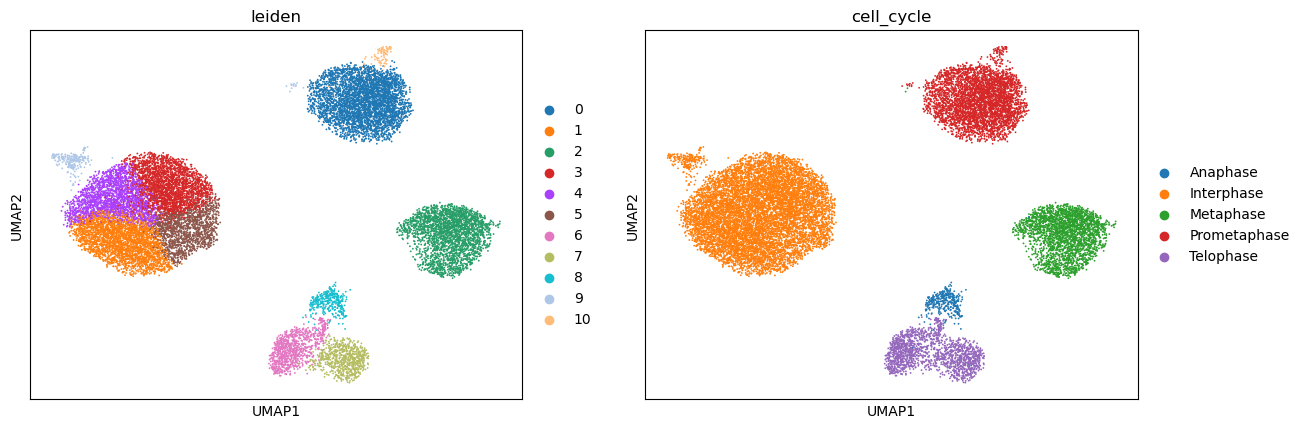
\includegraphics[width=\linewidth]{Figures/cellcycleclustering_afternca.png}
    \caption{Leiden clustering of Cell Cycle data following the distance metric learning algorithm NCA application.}
    \label{multifig4:image_c}
  \end{subfigure}
  \caption{Each figure represents data clustering, post the application of distance metric learning algorithm - NCA application.}
  \label{multifig4:DML_Clusters}
\end{figure}


Due to the same, it can be noticed that the information in / from the classical image features is not enough to form clusters of biological relevance.

\subsection{Pre-trained Deep Learning Models show inferior separation compared to classical image features}
The previously mentioned deep-learning models out-of-the-box were used to extract the features from the images. The performance of the models is mentioned in \ref{tab:performanceofdl} and \ref{multifig5:Outoftheboxclusters}.


\begin{table}[h]
\centering
\footnotesize
\caption{Performance of different pre-trained deep learning networks used to extract features from the images. The performance is measured using the cluster purity metric mentioned in \ref{cp}.}
\label{tab:performanceofdl}
\begin{tabular}{@{}p{1.8cm}cccccc@{}}
\toprule
\textbf{Deep Learning Network} & \multicolumn{2}{c}{\textbf{\textit{Salmonella}}} & \multicolumn{2}{c}{\textbf{Phytoplankton}} & \multicolumn{2}{c}{\textbf{Cell Cycle}} \\
% \cmidrule(r){2-3} \cmidrule(lr){4-5} \cmidrule(l){6-7}
& \textbf{Before NCA} & \textbf{After NCA} & \textbf{Before NCA} & \textbf{After NCA} & \textbf{Before NCA} & \textbf{After NCA} \\
\midrule
ResNet50 & 0.47567 & 0.47321 & 0.70098 & 0.70348 & 0.57469 & 0.61025 \\
ScDINO  & 0.52953 & 0.57076 & 0.59414 & 0.69794 & 0.54569 & 0.54789 \\
TransPath & 0.53083 & 0.53133 & 0.60485 & 0.63519 & 0.65229 & 0.71893 \\
\bottomrule
\end{tabular}
\end{table}



\begin{figure}
  \centering
  \begin{subfigure}{\linewidth}
    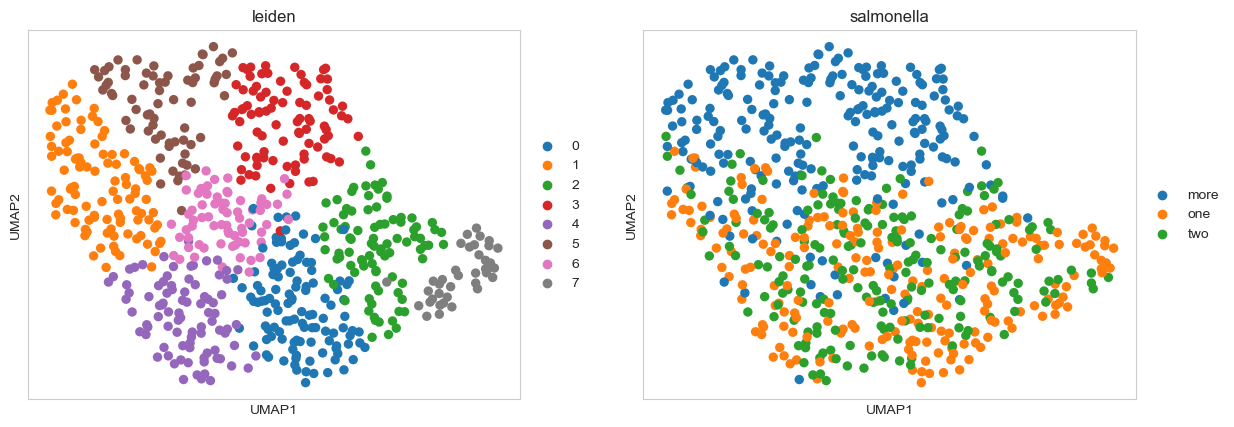
\includegraphics[width=\linewidth]{Figures/outoftheboxscDINOpostNCA_salmonella.png}
    \caption{Leiden clustering of \textit{Salmonella} data after the extraction of complex features from images using pre-trained network - scDINO and post NCA.}
    \label{multifig5:image_a}
  \end{subfigure}
  \hfill
  \begin{subfigure}{\linewidth}
    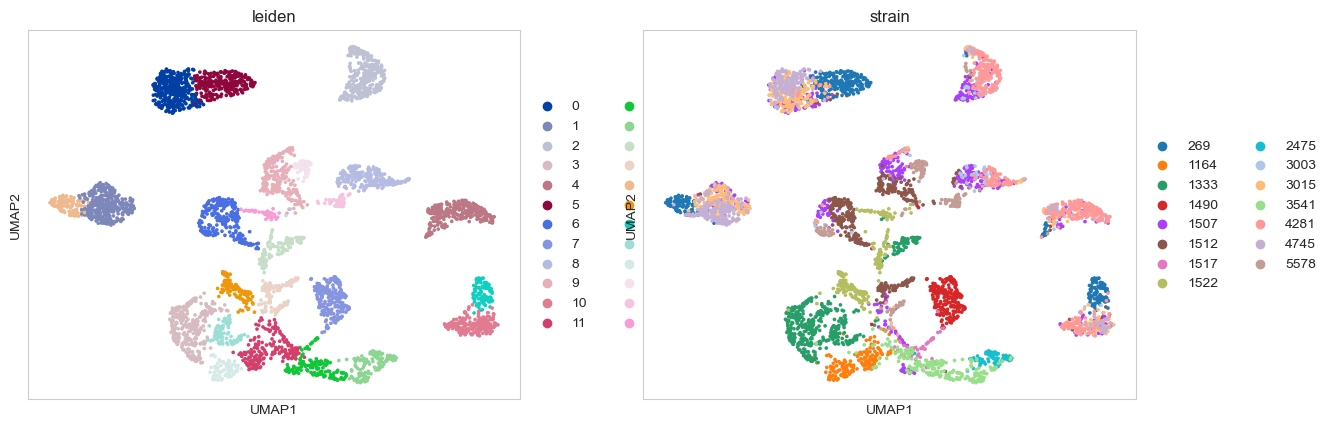
\includegraphics[width=\linewidth]{Figures/outoftheboxscDINOpostNCA_plankton.png}
    \caption{Leiden clustering of plankton data post extraction of complex features from images using pre-trained network - scDINO and post NCA.}
    \label{multifig5:image_b}
  \end{subfigure}
  \hfill
  \begin{subfigure}{\linewidth}
    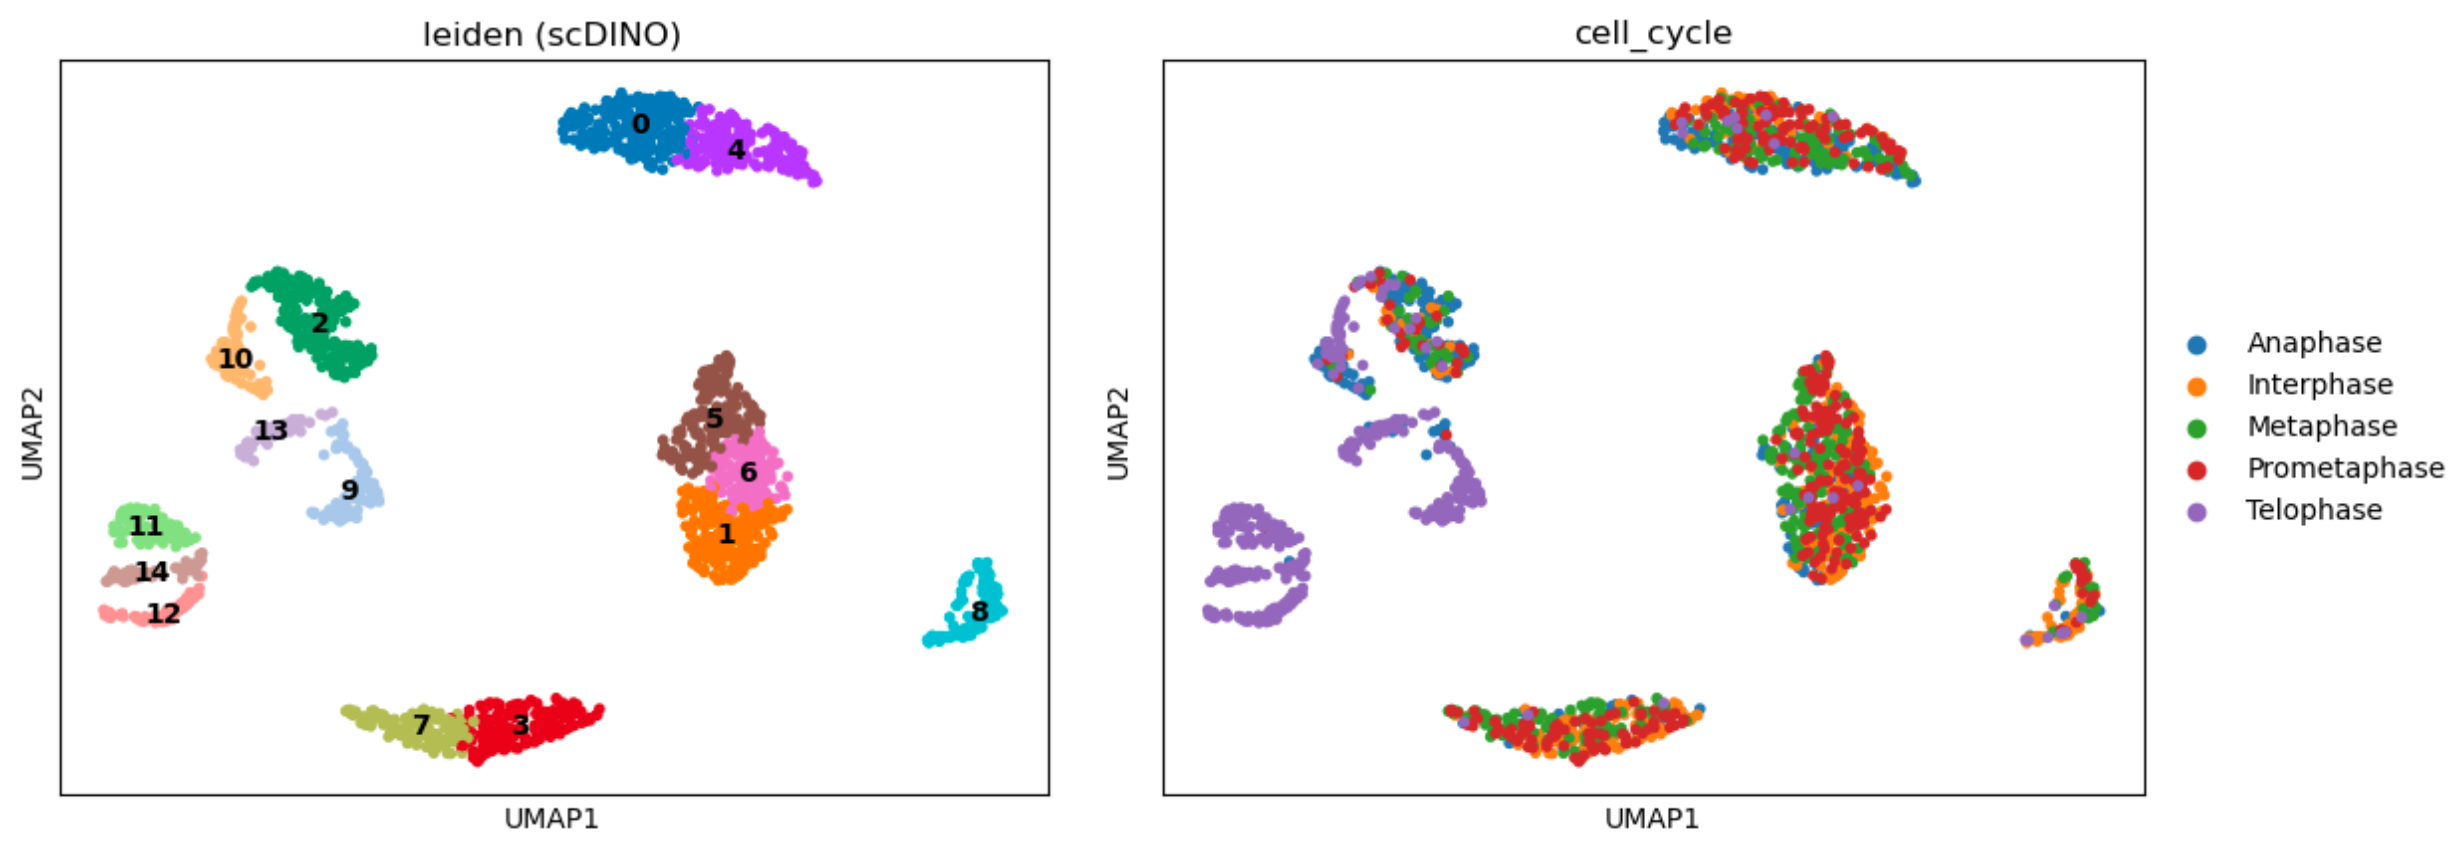
\includegraphics[width=\linewidth]{Figures/outoftheboxscDINOpostNCA_cellcycle.png}
    \caption{Leiden clustering of Cell Cycle data following the extraction of complex features from images using pre-trained network - scDINO, followed by NCA.}
    \label{multifig5:image_c}
  \end{subfigure}
  \caption{Each figure represents data clustering, post the application of distance metric learning algorithm - NCA application.}
  \label{multifig5:Outoftheboxclusters}
\end{figure}

%-----------

\subsection{Performance of scDINO Improved After Training}

The inferior performance of pre-trained deep learning models compared to classical features implies these generic networks have not learned feature representations tailored to this specific phenotypic clustering task. To address this, we trained the best performing out-of-the-box model, scDINO, on the full corpus of labeled and unlabelled images across the phytoplankton, \textit{Salmonella}, and cell cycle datasets. By training in an unsupervised manner on the combined datasets, we aimed to learn a specialized embedding optimized for our phenotypic clustering goal. The training loss decreased over epochs, indicating the model was learning from the diverse image data. After training, model weights were extracted and used to extract features from the images. However, clustering performance based on Neighborhood Components Analysis of the scDINO embeddings was still partially inferior compared to classical features, as shown in \ref{multifig6:ClustersaftertrainingscDINO} and \ref{tab:aftertrainingperformanceofscDINO}. While model training on relevant data improved over out-of-the-box features, tuning of the loss function, training procedure, and other optimizations may be needed to further focus learning on phenotypic differences critical for clustering performance.


\begin{figure}
  \centering
  \begin{subfigure}{\linewidth}
    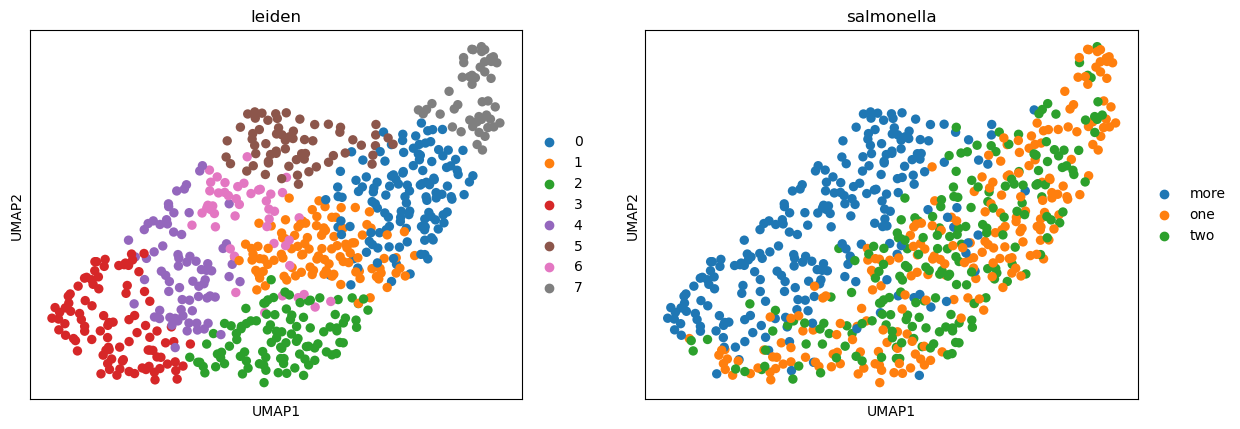
\includegraphics[width=\linewidth]{Figures/scDINOaftertrainingafterNCA_salmonella.png}
    \caption{Leiden clustering of \textit{Salmonella} data after the extraction of complex features from images after training scDINO on the \textit{Salmonella} dataset and post NCA.}
    \label{multifig6:image_a}
  \end{subfigure}
  \hfill
  \begin{subfigure}{\linewidth}
    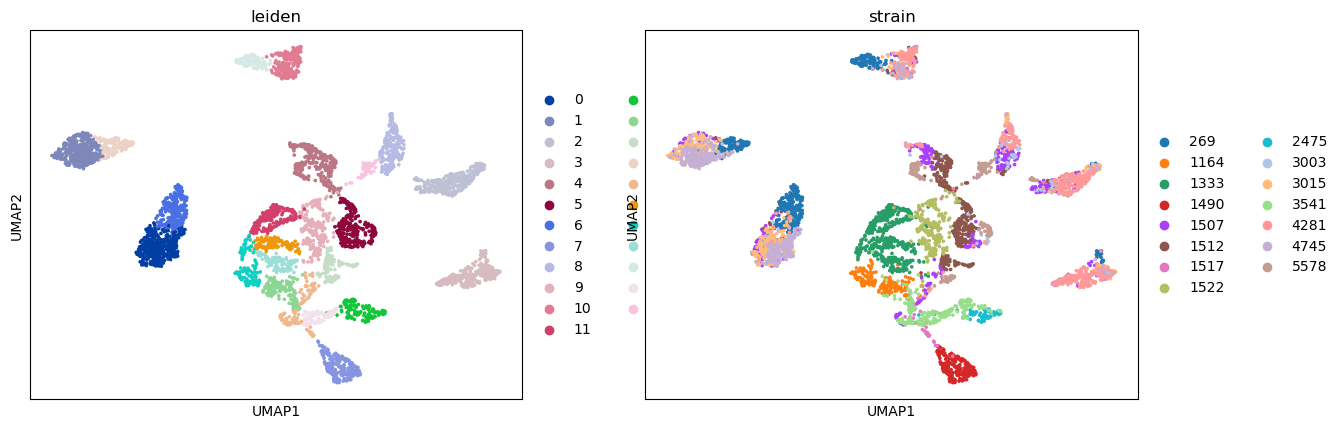
\includegraphics[width=\linewidth]{Figures/scDINOaftertrainingafterNCA_plankton.png}
    \caption{Leiden clustering of plankton data post the extraction of complex features from images after training scDINO on the plankton dataset, followed by NCA.}
    \label{multifig6:image_b}
  \end{subfigure}
  \hfill
  \begin{subfigure}{0.3\linewidth}
    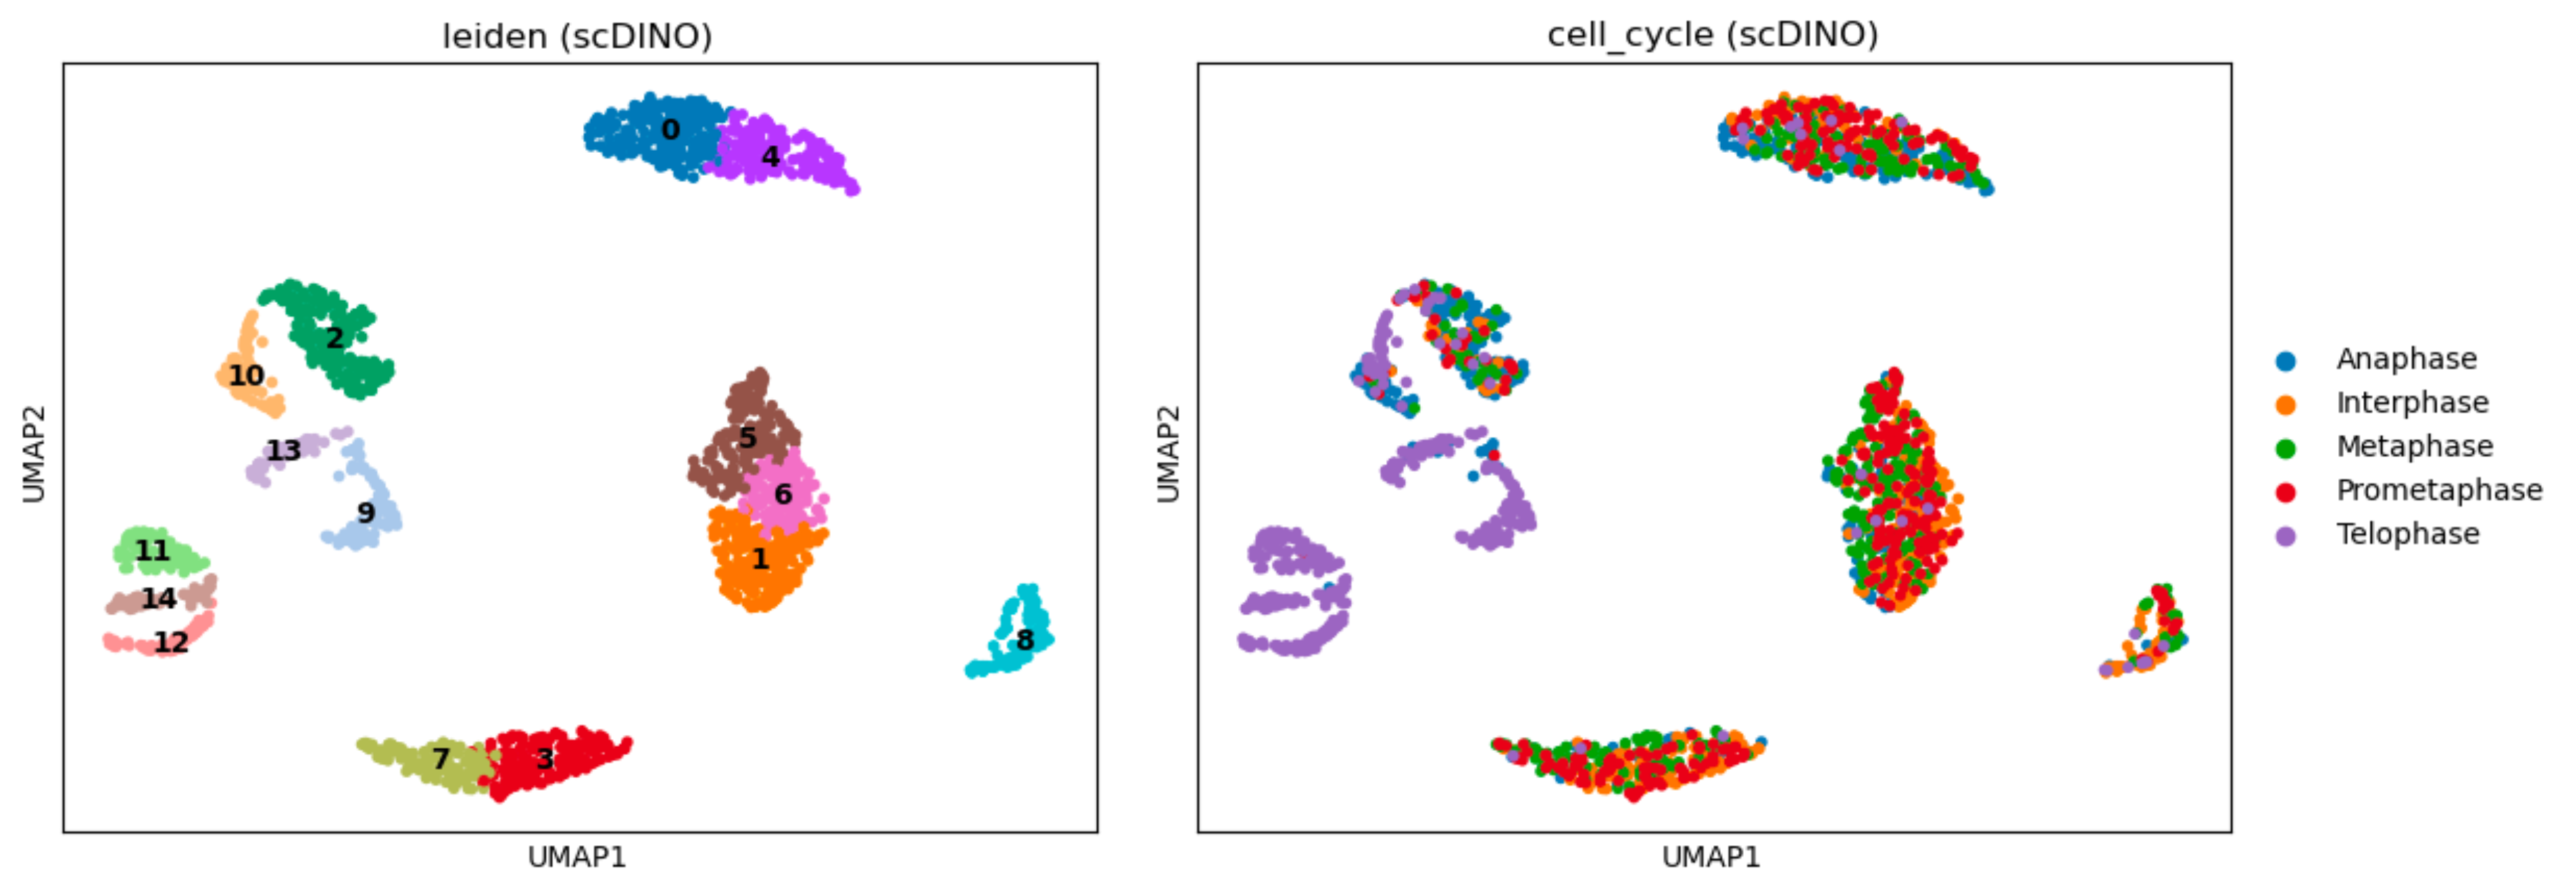
\includegraphics[width=0.3\linewidth]{DineshPalliMasterThesis/Figures/scDINOaftertrainingafterNCA_cellcycle.png}
    \caption{Leiden clustering of Cell Cycle data following the extraction of complex features from images after training scDINO on the cellcycle dataset and post NCA.}
    \label{multifig6:image_c}
  \end{subfigure}
  \caption{Each figure represents data clustering, post training and post application of distance metric learning algorithm - NCA application.}
  \label{multifig6:ClustersaftertrainingscDINO}
\end{figure}


\begin{table}[h]
\centering
\small
\caption{Table showing the performance of scDINO deep learning network after training, used to extract features from the images. The performance is measured using the cluster purity metric mentioned in \ref{cp}.}
\begin{tabular}{|>{\raggedright\arraybackslash}p{2.5cm}|*{4}{>{\raggedright\arraybackslash}p{1.9cm}|}}
\hline
\textbf{Deep Learning Network} & \multicolumn{2}{c|}{\textbf{Salmonella Dataset}} & \multicolumn{2}{c|}{\textbf{Phytoplankton Dataset}} & \multicolumn{2}{c|}{\textbf{Cell Cycle Dataset}} \\
\cline{2-7}
 & \textbf{Before NCA} & \textbf{After NCA} & \textbf{Before NCA} & \textbf{After NCA} & \textbf{Before NCA} & \textbf{After NCA} \\ 
\hline
\textbf{ScDINO} & 0.46939 & 0.62408 & 0.61468 & 0.67523 & & & & \\
\hline
\end{tabular}
\label{tab:aftertrainingperformanceofscDINO}
\end{table}
%-----------
\par\hspace{2cm} 
\newpage

\section{Discussion}
\label{Discussion}
\input{chapters/discussion}

Advances in microscopy and imaging technologies have enabled the collection of high-dimensional data across diverse biological contexts. However, making full use of these rich datasets poses challenges for traditional analysis approaches. As image volumes grow, manual analysis becomes infeasible, requiring more automated computational solutions to identify relevant features and patterns. In this regard, deep learning has shown immense promise for bioimage analysis, demonstrating high performance on tasks like segmentation, classification, and clustering. By learning complex feature representations directly from pixel data, neural networks can capture subtle morphologies and textures in cell images that are valuable for understanding variations in cell type and state. In this study, we aimed to develop a deep learning-based embedding that can disentangle complex image features relevant to cell-type and state variation from high-dimensional ICS data. Our goal was to enable biologically meaningful clustering of single cells in an unsupervised, unbiased manner, which could be applied across diverse datasets from multiple experiments. We evaluated whether classical image features contain enough information for effective clustering, or if more complex embeddings learned via deep neural networks on images are required. We tested dimensionality reduction and clustering methods on classical features, applied distance metric learning to transform the feature space, and analyzed pre-trained deep learning models for their embedding performance. We also trained the deep learning networks on our data, to evaluate their performance.

The results presented indicate that relying solely on classical image features is insufficient for forming biologically meaningful clusters across the diverse datasets - \textit{Salmonella}, phytoplankton, and cell cycle images. While these features provide a preliminary separation between some states, they lack the complexity and discriminative power to finely differentiate between subtle phenotypic differences that denote variations in cell type or condition. This can be seen in \cite{multifigure3:overall_figure}. Some reasons why this occurred might be capacity of hand-engineered features to not capture the intricate textural, shape, and morphological characteristics that distinguish cell phenotypes of the cells. Moreover, the classical image features are designed generically and not specific to the individual datasets. But the cluster purity of the cell cycle data was higher than other datasets. Light scattering profiles have been closely correlated to the nuclear morphology and changes during cell cycle \cite{WOS:A1974T155500001, benson_mcdougal_coffey_1984}. Nuances in the staining patterns, spatial protein distributions, and textural motifs within cells, which are specific to dataset (cells and their morphology) are unlikely to be encoded by classical features.

The histograms comparing feature distributions before and after scaling (Figures 3 and 4) demonstrate that scaling can help amplify the differences between clusters to some extent. This scaling has proved that the clusters can be separated, in the case of som phytoplankton strains. However, this amplification is modest, and several strains still exhibit significant overlap even after scaling. For instance, in the phytoplankton data, strains 1512, 3003 and 4281 remain blended together post-scaling. Similarly, the\textit{Salmonella} clusters denoting one vs two bacteria per cell show little separation following scaling. But for inseparable clusters, the differences may be more subtle and not well captured by the classical features even after scaling. In relation to the plankton biology, the composition of the culture medium is another critical factor to consider when isolating phytoplankton strains. Despite the potential effects that different media may have on the success of phytoplankton isolation and growth, few studies have systematically evaluated the impacts of various media formulations. Harrison and Berges (2005) quoted McLachlan (1973): 'Numerous enriched and synthetic media have been formulated, which together with generally trivial modifications, almost equal the number of investigators' \cite{HarrisonPaul}. Cells infected with \textit{Salmonella} have one, two or more \textit{Salmonella} inside. Cells with more \textit{Salmonella} show high intensity than the cells with one or two \textit{Salmonella} inside them. When the \textit{Salmonella} is multiplying inside the cell, there is change in the pixel area over time, which is useful for the clustering, but the size of \textit{Salmonella} is relatively small in comparison to the cell and the ICS captures the features of the entire cell \cite{fàbrega_vila_2013}. As the \textit{Salmonella} multiply the intensity of the fluorescence increase in the cell, and this can also be noticed as the cluster with more \textit{Salmonella} is relatively more isolated from clusters with one and two \textit{Salmonellae} inside them \ref{multifig1:image_a}. In the case of cells with one or two \textit{Salmonellae}, during the bacterial reproduction, the fluorescent signals might be close to each other during separation. This can result in an elongated spot of fluorescence, rather than two different spots resulted from completion of multiplication of the bacterium. Capturing more details by the ICS, in the case of \textit{Salmonella} data, including the non-biologically relevant data, from the cells encapsulating the bacteria, which makes it difficult to infer the biologically relevant features. This can also be noticed from the complex features extracted from the images.

This implies that while scaling transforms the range of feature values to highlight differences, the features themselves do not fully encapsulate the intrinsic characteristics that demarcate distinct cell types in this data. More complex features are needed to delineate boundaries between biologically meaningful groups.

Applying dimensionality reduction techniques like PCA and UMAP visualization directly on the classical features provides some preliminary clusters, but many are indistinguishable (Figure 1). For example, in the \textit{Salmonella} data, clusters representing one bacterium per cell versus two bacteria per cell are not differentiated clearly. This indicates the classical features do not adequately capture morphological differences between these phenotypes.

Using distance metric learning algorithms like NCA on the features improves purity (cluster accuracy) to some degree but still does not lead to a complete separation of relevant biological groups (Table 1, Figure 5). Some cell type clusters remain mixed, like those seen earlier. There are two reasons that might have caused this, one, the cell cycle consists of fixed progression of stages that cells pass through sequentially. Each stage has distinct phenotype that is reflected in the cells. But the transitions between adjacent phases are gradual. Cells entering a new phase retain remnants of the prior one.
This means proximate cell cycle stages are intrinsically more similar than distant stages. Distance Metric Learning (DML) can take advantage of this inherent structure by pulling closer points near each other in the progression while pushing apart distant phases. Essentially, DML is able to embed information about the sequential ordering of the cycle into the transformed feature space. DML techniques like NCA learn linear transformations of the feature space \cite{NCA}. The phenotypic differences across cell cycle phases follow observable patterns in size, shape etc. These morphological changes can likely be captured through linear feature transformations. But for the \textit{Salmonella} and phytoplankton data, discriminative patterns are likely more complex and non-linear. In case of \textit{Salmonella}, the bacteria might be small and the differences subtle to capture biologically relevant information. The physiology of the plankton changes from strain to strain and some strains could possibly be similar to each other with subtle feature differences. Simple linear transformations are insufficient to disentangle these complex feature relationships. Datasets with gradual, ambiguous differences require learning highly non-linear mappings from features to phenotypes. These datasets (salmonella and plankton), because of their variations demand complex non-linear feature dependencies that linear DML cannot represent. In contrast, the more structured cell cycle changes are amenable to linear separations, explaining DML's success. This orderly alignment and natural similarities between adjoining phases likely explains why DML was effective for cell cycle separation. NCA performed better than other DML algorithms, because as a probabilistic model, it is less prone to overfitting compared to margin-based techniques like LMNN, especially with limited training data. NCA is designed to optimize leave-one-out classification accuracy directly, whereas other methods optimize different proxy objectives like relative distances or margins between classes. This may have made NCA better suited for our classification-focused goal.

The dataset formed by merging the three datasets, did not perform any better and it is justified as there are many features to learn from and some of the features from different datasets are overlapping and might conflict with each other which hinders the formation of biologically relevant clusters \ref{<Reference>}.

The inferior performance of pre-trained deep learning models compared to classical features (\ref{tab:performanceofdl}) implies these generic networks have not learned feature representations tailored to this specific phenotypic clustering task when used out-of-the-box. Their internal representations may not fully disentangle the properties critical for phenotype-based clustering. Models like ResNet50, scDINO and TransPath were pre-trained on natural image datasets like ImageNet or histopathology data. They have not seen enough relevant cell images to learn features optimized for differentiating cell types and states based on their morphology. scDINO was trained on single cell data, which is similar to our datasets \ref{scdinoworking}. ScDINO learns both local patterns within image patches and global context from the full image via the vision transformer architecture. This multi-scale representation may have aided clustering. Also, all the three networks used performed inferiorly on the \textit{Salmonella} data. This can also be due to the small size of the labelled data, which is 655 images, typically considered very small for a neural network.

Taken together, these results strongly indicate that while classical features and scaling provide a partial separation between some states, they lack the complexity and dimensionality needed to finely discriminate between subtle biological variations that correspond to changes in cell type or condition. Pre-trained deep learning models also do not readily learn feature spaces conducive for this goal without explicit training on relevant data. This strongly motivates the need for learning specialized embeddings tailored to the specific task of phenotypic clustering. The generic embeddings derived from pre-trained models are unlikely to effectively disentangle the intricate combination of morphological features that denotes variations in cell type and state without dedicated training on such data. 

A deep neural network trained in an end-to-end fashion on diverse datasets spanning different cell types, states, and conditions may potentially learn a rich, high-dimensional embedding space capable of separating clusters belonging to distinct phenotypes. For the same, we trained the scDINO network on our data to evaluate the performance of the network after training. For the same, we first trained the network on datasets separately to evaluate the individual increment in performance. To our surprise, the trained models performed relatively better when compared with pre-trained network and performed inadequately compared with DML. This could possibly be due to the capturing all the features of the images both biologically relevant and non-relevant. This can be especially true in relation to \textit{Salmonella} dataset as the details that are biologically relevant are the ones in bacteria, which is actually a minor part of the entire image of the cell. But the network tends to learn all the features of the cell too. But with plankton, the performance improved on average, relatively as the strains look different from each other morphologically. Some strains which tend to look similar are not clearly separated when the clusters are formed as can be seen in \ref{multifig6:ClustersaftertrainingscDINO}.

Cluster purity was utilized as metric to evaluate the quality of clusters generated by the clustering algorithms in our work. Cluster purity provides a measure of how well clusters map to single classes, by calculating the percentage of samples assigned to their dominant class in each cluster. A purity score of 1 indicates perfectly separated clusters with no mixing of data from different classes.

While cluster purity gives an intuitive sense of cluster accuracy, it is seldom perfect. Purity can be biased by imbalanced dataset sizes, and does not penalize having redundant or excessive clusters. Further, purity only considers the dominant class in each cluster, ignoring potential mixing of other classes. For the same reason, we recommend future studies involving complex extrinsic metrics (requires ground truth labels) namely, Adjusted Rand Index (ARI), Normalised Mutual Information (NMI), Fowlkes-Mallows Index (FMI) and intrinsic metrics (do not require ground truth labels) viz., Silhouette Coefficient, Calinski-Harabasz Index, Davies-Bouldin Index. It is recommended to use both ADI or NMI and Silhouette Coefficient as both ADI and NMI account for random chance in cluster assignment which makes it more robust \cite{ARI, NMI}. Combining it with Silhouette Coefficient which quantifies how the points in a cluster are tightly grouped compared with other clusters provides additional information beyond accuracy \cite{silhouettecoefficient}. Both the metrics are commonly used and well-known in the literature which makes them easier to interpret too.

\textbf{Adjusted Rand Index (ARI)}
\begin{equation}
\text{ARI} = \frac{\sum_{ij} \binom{n_{ij}}{2} - \biggl[ \sum_i \binom{a_i}{2}  \sum_j \binom{b_j}{2} \biggr] / \binom{n}{2}} {\frac{1}{2} \biggl[ \sum_i \binom{a_i}{2} + \sum_j \binom{b_j}{2} \biggr] - \biggl[ \sum_i \binom{a_i}{2}  \sum_j \binom{b_j}{2} \biggr] / \binom{n}{2}}
\end{equation}

% \textbf{Adjusted Rand Index (ARI)}
% \begin{equation}
% \text{ARI} = \frac{\sum_{ij} \binom{n_{ij}}{2} - \bigl[\sum_i \binom{a_i}{2} \sum_j \binom{b_j}{2} \bigr] / \binom{n}{2}} {\frac{1}{2} \bigl[\sum_i \binom{a_i}{2} + \sum_j \binom{b_j}{2} \bigr] - \bigl[\sum_i \binom{a_i}{2} \sum_j \binom{b_j}{2} \bigr] / \binom{n}{2}}  
% \end{equation}

Where $n_{ij}$ is the number of samples assigned to cluster $i$ in the first clustering and cluster $j$ in the second clustering. $a_i$ and $b_j$ are the totals for cluster $i$ and $j$ respectively \cite{ARI}.

\textbf{Normalized Mutual Information (NMI)}
\begin{equation}
\text{NMI}(Y, C) = \frac{2 I(Y;C)}{[H(Y) + H(C)]}
\end{equation}

Where $Y$ are the true labels, $C$ are the predicted clusters, $I(Y;C)$ is their mutual information, and $H$ is entropy \cite{NMI}.

\textbf{Silhouette Coefficient}
\begin{equation}
s = \frac{b-a}{\max(a,b)}
\end{equation}

Where $a$ is the mean intra-cluster distance and $b$ is the nearest cluster distance for each sample. The score is averaged over all samples \cite{silhouettecoefficient}.


Further improvements to the disentangling of complex features extracted from the images can be done, with slightly changing the loss function. Combining the contrastive loss with cluster separation loss would improve the separation of clusters and improve the accuracy. Using a contrastive loss like Normalized Temperature-scaled Cross Entropy Loss (NT-Xent) over cross entropy could better capture similarities between images of the same phenotype \cite{koch2015siamese}. NT-Xent is more robust to noise and is a metric learning approach. It operates on both pairs or triplets of samples which suits to Salmonella dataset. Additionally, it can be combined with cluster separation loss, since it penalises the cluster centroids to push entire clusters away from each other \cite{xu2018variational}. This combination helps the network learn fine similarities in local samples (with contrastive loss) and higher level inter-cluster relations (with cluster separation loss). We have not tried DINO2, the latest update to the DINO, proven to perform better than DINOv1, with improved attention mechanism, which could also be trained and tried on our data \cite{chen2023dinov2}.

\begin{equation}
\mathcal{L}{hybrid} = \mathcal{L}{NT-Xent} + \lambda \mathcal{L}_{separation}
\end{equation}

Where:

\begin{equation}
\mathcal{L}{NT-Xent} = - \frac{1}{N} \sum{i=1}^N \log \frac{\exp(x_i \cdot x_j / \tau)}{\sum_{k \neq i} \exp(x_i \cdot x_k / \tau)}
\end{equation}

is the NT-Xent loss between positive pairs $(i,j)$,

and the cluster separation loss is defined as:

\begin{equation}
\mathcal{L}{separation} = \sum{c_1 \neq c_2} \max(0, m - D(c_1, c_2))
\end{equation}

which applies a margin $m$ between the centroids $c_1$ and $c_2$ of different clusters, with $D$ measuring the distance.

The hyperparameter $\lambda$ balances the two loss components. This hybrid formulation allows jointly modeling sample similarity with NT-Xent and cluster separation.

In addition to adjusting the loss function, training regime can be fine-tuned for optimal performance including, oversampling labeled images during training to focus learning on phenotypic differences. Unlabelled images can be used for pre-training then fine-tuned on labeled data. Curriculum learning approach can be tried, by starting with easy separations then progressively make clustering harder as training improves \cite{bengio2009curriculum}. Two-stage training could be attempted, where the model is first trained on all data, then fine-tuned on labeled subsets for phenotypically relevant features. Providing class/phenotype labels during training to directly optimizes the embedding for clustering rather than only reconstruction.

In this study, we showed that the possibility that clustering can be performed with DML and deep neural networks. While classical features and generic deep learning embeddings provided preliminary cluster separations, neither fully captured the nuanced morphological patterns distinguishing cell types and states. However, by training a vision transformer end-to-end on diverse biological datasets, we demonstrated deep learning's potential to learn tailored representations needed to finely discriminate phenotypes once tuned on relevant data. Further optimizations to the loss function, training procedure, and network architecture could better focus learning on biologically-meaningful traits. Overall, this study highlighted both the challenges and prospects of automated phenotypic characterization from images using deep neural networks. With problem-specific tuning, we are optimistic deep learning can reveal new phenotypic relationships within complex cellular populations in an unbiased manner.

\newpage

% ------------------------------------------------------------------------------
% APPENDIX ---------------------------------------------------------------------
% ------------------------------------------------------------------------------
    
%\pagenumbering{Roman}
%
%\setcounter{page}{5} % CHANGE
%
%\appendix
%
%\section{Appendix}
%\label{app}
%\input{chapters/appendix}
%\newpage
%
%\section{Electronic appendix}
%\label{el_app}
%
%Data, code and figures are provided in electronic form.
%
%\newpage
    
% ------------------------------------------------------------------------------
% BIBLIOGRAPHY -----------------------------------------------------------------
% ------------------------------------------------------------------------------

\RaggedRight
\bibliography{bibliography}
\bibliographystyle{unsrt}
\newpage

\newpage

\section{Acknowledgement}
\label{Acknowledgement}

First and foremost, I would like to express my deepest gratitude to my principal investigator, \mysupervisor{}, and my internal supervisor, \myinternalsupervisor{}, for their guidance and for examining my thesis. Their expertise and insights have been invaluable to my academic journey.
\paragraph{}
I am particularly indebted to my supervisor, Louis Kümmerlee, who has provided constant support throughout this process. His patience, knowledge, and being a Swiss Army Knife in answering all my queries and doubts has been instrumental in the completion of this thesis. He was always there for me when needed, and for that, I am truly grateful.
\paragraph{}
I would also like to extend my thanks to my lab members, especially Felix Fischer and Giovanni Palla, among others. Their support and camaraderie have made this journey a happy, rewarding and enriching experience.
\paragraph{}
On a personal note, I wish to express my heartfelt gratitude to my family: my parents, Madhava Reddy Palli and Samrajya Lakshmi Kalluru, and my brother, Sai Swaroop Palli. They have been my pillars of strength, providing unwavering support and encouragement throughout my academic journey and through life.
\paragraph{}
I am profoundly indebted to my friends, Atharv Arora, Shrey Parikh, Krishna Sai, Divya and Bhavna Menon. During the times when I found myself in the deepest valleys of my journey, they were there, ready to jump-start my faltering spirit with their unwavering belief in me. Their friendship has been more than just a source of camaraderie; it has been a beacon of hope in my darkest hours. The emotional support they provided has been my anchor, grounding me when the storms of doubt threatened to carry me away. Their presence in my life is a gift I will forever cherish.
\paragraph{}
In the grand tradition of alphabetical order, I extend my heartfelt thanks to Aarushi Davesar, Sabeel Un Naeem, and Siddhi Pawar. You have been my personal cheerleading squad, my stress relief hotline, and my partners in laughter. Thank you for being the 'safety valves' for my occasional steam-letting sessions and for standing by me when life decided to play limbo. Your unwavering positivity and constant encouragement have been the lighthouse guiding me through the foggy nights of this academic journey. For that, I owe you a debt of gratitude... and perhaps a round of ice cream!
\paragraph{}
In conclusion, I recognize that this achievement would not have been possible without the support, guidance, and encouragement of each individual mentioned above, and for this, I am eternally grateful.


% ------------------------------------------------------------------------------
% DECLARATION OF AUTHORSHIP & ORIGINALITY-----------------------------------------------------
% ------------------------------------------------------------------------------
\clearpage

\includepdf{Attachments/master_thesis_last_page.pdf}
\addcontentsline{toc}{chapter}{Statement of Originality}

%\Large
%\noindent
%\textbf{Declaration of authorship}
%\vspace{0.5cm}
%\noindent
%\normalsize
%
%I hereby declare that the report submitted is my own unaided work. All direct 
%or indirect sources used are acknowledged as references. I am aware that the 
%Thesis in digital form can be examined for the use of unauthorized aid and in 
%order to determine whether the report as a whole or parts incorporated in it may 
%be deemed as plagiarism. For the comparison of my work with existing sources I 
%agree that it shall be entered in a database where it shall also remain after 
%examination, to enable comparison with future Theses submitted. Further rights 
%of reproduction and usage, however, are not granted here. This paper was not 
%previously presented to another examination board and has not been published.
%\\
%
%\vspace{1cm}
%Munich, January 30\textsuperscript{th}, 2023
%
%\textcolor{orange}{Location, date} \\
%
%\vspace{3cm}
%
%Dinesh Reddy Palli
%
%\noindent\rule{0.5\textwidth}{0.4pt} \\
%
%\textcolor{orange}{Name}

% ------------------------------------------------------------------------------

\end{document}
